% A LaTeX template for MSc Thesis submissions to 
% Politecnico di Milano (PoliMi) - School of Industrial and Information Engineering
%
% S. Bonetti, A. Gruttadauria, G. Mescolini, A. Zingaro
% e-mail: template-tesi-ingind@polimi.it
%
% Last Revision: October 2021
%
% Copyright 2021 Politecnico di Milano, Italy. NC-BY

\documentclass{config/PoliMi3i_thesis}

%------------------------------------------------------------------------------
%	REQUIRED PACKAGES AND  CONFIGURATIONS
%------------------------------------------------------------------------------

% Uncomment to show margins
%\usepackage{showframe}

% PACKAGE FOR CUSTOM LISTS
\usepackage{enumitem}

% CONFIGURATIONS
\usepackage{parskip} % For paragraph layout
\usepackage{setspace} % For using single or double spacing
\usepackage{emptypage} % To insert empty pages
\usepackage{multicol} % To write in multiple columns (executive summary)
\setlength\columnsep{15pt} % Column separation in executive summary
\setlength\parindent{0pt} % Indentation
\raggedbottom

% PACKAGES FOR TITLES
\usepackage{titlesec}
% \titlespacing{\section}{left spacing}{before spacing}{after spacing}
\titlespacing{\chapter}{0pt}{0ex}{8ex}
\titlespacing{\section}{0pt}{3.3ex}{2ex}
\titlespacing{\subsection}{0pt}{3.3ex}{1.65ex}
\titlespacing{\subsubsection}{0pt}{3.3ex}{1ex}
\usepackage{color}

% PACKAGES FOR LANGUAGE AND FONT
\usepackage[english]{babel} % The document is in English  
\usepackage[utf8]{inputenc} % UTF8 encoding
\usepackage[T1]{fontenc} % Font encoding
\usepackage[11pt]{moresize} % Big fonts

% PACKAGES FOR IMAGES
\usepackage{graphicx}
\usepackage{transparent} % Enables transparent images
\usepackage{eso-pic} % For the background picture on the title page
\usepackage{subfig} % Numbered and caption subfigures using \subfloat.
\usepackage{tikz} % A package for high-quality hand-made figures.
\usetikzlibrary{}
\graphicspath{{./images/}} % Directory of the images
\usepackage{caption} % Coloured captions
\usepackage{xcolor} % Coloured captions
\usepackage{amsthm,thmtools,xcolor} % Coloured "Theorem"
\usepackage{float}
\ifdefined\emitpumldiagrams{}
    \usepackage{svg} % svgs
    \pdfsuppresswarningpagegroup=1 % disable svg export warnings
\fi
\usepackage{adjustbox} % adjust svg size to fit
 
% STANDARD MATH PACKAGES
\usepackage{amsmath}
\usepackage{amsthm}
\usepackage{amssymb}
\usepackage{amsfonts}
\usepackage{bm}
\usepackage[overload]{empheq} % For braced-style systems of equations.
\usepackage{fix-cm} % To override original LaTeX restrictions on sizes

% PACKAGES FOR TABLES
\usepackage{tabularx}
\usepackage{longtable} % Tables that can span several pages
\usepackage{colortbl}
\usepackage{multirow}
\setlength\LTpost{-3.5em}

% PACKAGES FOR ALGORITHMS (PSEUDO-CODE)
\usepackage{algorithm}
\usepackage{algorithmic}
\usepackage{listings}
\usepackage{config/alloy-style}

% PACKAGES FOR REFERENCES & BIBLIOGRAPHY
\PassOptionsToPackage{hyphens}{url}
\usepackage[colorlinks=true,linkcolor=black,anchorcolor=black,citecolor=black,filecolor=black,menucolor=black,runcolor=black,urlcolor=black]{hyperref} % Adds clickable links at references
\usepackage{cleveref}
\usepackage[square, numbers, sort&compress]{natbib} % Square brackets, citing references with numbers, citations sorted by appearance in the text and compressed
\bibliographystyle{abbrvnat}

% OTHER PACKAGES
\usepackage{pdfpages} % To include a pdf file
\usepackage{afterpage}
\usepackage{lipsum} % DUMMY PACKAGE
\usepackage{fancyhdr} % For the headers
\usepackage{tabu}
\usepackage[]{underscore} % To be able to use _ in text
\fancyhf{}

% Input of configuration file. Do not change config.tex file unless you really know what you are doing. 
% !TeX root = ../rasd.tex
% Define blue color typical of polimi
\definecolor{bluepoli}{cmyk}{0.4,0.1,0,0.4}

% Custom theorem environments
\declaretheoremstyle[
  headfont=\color{bluepoli}\normalfont\bfseries,
  bodyfont=\color{black}\normalfont\itshape,
]{colored}

% Set-up caption colors
\captionsetup[figure]{labelfont={color=bluepoli}} % Set colour of the captions
\captionsetup[table]{labelfont={color=bluepoli}} % Set colour of the captions
\captionsetup[algorithm]{labelfont={color=bluepoli}} % Set colour of the captions

\theoremstyle{colored}
\newtheorem{theorem}{Theorem}[chapter]
\newtheorem{proposition}{Proposition}[chapter]

% Enhances the features of the standard "table" and "tabular" environments.
\newcommand\T{\rule{0pt}{2.6ex}}
\newcommand\B{\rule[-1.2ex]{0pt}{0pt}}

% Pseudo-code algorithm descriptions.
\newcounter{algsubstate}
\renewcommand{\thealgsubstate}{\alph{algsubstate}}
\newenvironment{algsubstates}
{\setcounter{algsubstate}{0}%
  \renewcommand{\STATE}{%
    \stepcounter{algsubstate}%
    \Statex {\small\thealgsubstate:}\space}}
{}

% New font size
\newcommand\numfontsize{\@setfontsize\Huge{200}{60}}

% Title format: chapter
\titleformat{\chapter}[hang]{
  \fontsize{50}{20}\selectfont\bfseries\filright}{\textcolor{bluepoli} \thechapter\hsp\hspace{2mm}\textcolor{bluepoli}{|   }\hsp}{0pt}{\huge\bfseries \textcolor{bluepoli}
}

% Title format: section
\titleformat{\section}
{\color{bluepoli}\normalfont\Large\bfseries}
{\color{bluepoli}\thesection.}{1em}{}

% Title format: subsection
\titleformat{\subsection}
{\color{bluepoli}\normalfont\large\bfseries}
{\color{bluepoli}\thesubsection.}{1em}{}

% Title format: subsubsection
\titleformat{\subsubsection}
{\color{bluepoli}\normalfont\large\bfseries}
{\color{bluepoli}\thesubsubsection.}{1em}{}

% Shortening for setting no horizontal-spacing
\newcommand{\hsp}{\hspace{0pt}}

\makeatletter
% Renewcommand: cleardoublepage including the background pic
% \renewcommand*\cleardoublepage{%
%   \clearpage\if@twoside\ifodd\c@page\else
%       \null
%       \AddToShipoutPicture*{\BackgroundPic}
%       \thispagestyle{empty}%
%       \newpage
%       \if@twocolumn\hbox{}\newpage\fi\fi\fi}
% To avoid that LaTeX forces chapters to start always on even pages
\renewcommand{\cleardoublepage}{\clearpage}
\makeatother

%For correctly numbering algorithms
\numberwithin{algorithm}{chapter}

%----------------------------------------------------------------------------
%	NEW COMMANDS DEFINED
%----------------------------------------------------------------------------

\newcommand*{\puml}[2][]{%
    \ifdefined\emitpumldiagrams{}
        \immediate\write18{./puml/compile-svg.sh #2}
        \begin{adjustbox}{max size={\textwidth}{\textheight}}
            % inkscapelatex false cause otherwise for some reason inkscape puts white boxes all around text
            \includesvg[inkscapelatex=false, #1]{#2}%
        \end{adjustbox}
    \fi
}

\newcommand*{\textheightwithcaption}[1]{%
    \dimexpr\textheight
    -\parskip%
    -\abovecaptionskip%
    -\belowcaptionskip%
    -(\baselineskip*#1)\relax
}

\newcommand*{\labelleditem}[1]{
    \item \expandafter\gdef\csname \theenumi\endcsname{#1} \label{\theenumi} #1
}

\newcommand*{\labelledsubitem}[1]{
    \item \expandafter\gdef\csname \theenumii\endcsname{#1} \label{\theenumii} #1
}

\newcommand{\printitem}[1] {
	\item[\textbf{\ref{{#1}}}:] \csname {#1}\endcsname
}


% EXAMPLES OF NEW COMMANDS
\newcommand{\bea}{\begin{eqnarray}} % Shortcut for equation arrays
\newcommand{\eea}{\end{eqnarray}}
\newcommand{\e}[1]{\times 10^{#1}}  % Powers of 10 notation

%----------------------------------------------------------------------------
%	ADD YOUR PACKAGES (be careful of package interaction)
%----------------------------------------------------------------------------

%----------------------------------------------------------------------------
%	ADD YOUR DEFINITIONS AND COMMANDS (be careful of existing commands)
%----------------------------------------------------------------------------

% Some utilities\ldots
\newcommand{\comment}[1]{{\color{red}\(\blacktriangleright\) Comment: #1 \(\blacktriangleleft\)}}
\usepackage{soul}
\usepackage{tikz}

\usetikzlibrary{calc}
\usetikzlibrary{decorations.pathmorphing}


\makeatletter

\newcommand{\defhighlighter}[3][]{%
  \tikzset{every highlighter/.style={color=#2, fill opacity=#3, #1}}%
}

\defhighlighter{yellow}{.5}

\newcommand{\highlight@DoHighlight}{
  \fill [ decoration = {random steps, amplitude=1pt, segment length=15pt}
        , outer sep = -15pt, inner sep = 0pt, decorate
       , every highlighter, this highlighter ]
        ($(begin highlight)+(0,8pt)$) rectangle ($(end highlight)+(0,-3pt)$) ;
}

\newcommand{\highlight@BeginHighlight}{
  \coordinate (begin highlight) at (0,0) ;
}

\newcommand{\highlight@EndHighlight}{
  \coordinate (end highlight) at (0,0) ;
}

\newdimen\highlight@previous
\newdimen\highlight@current

\DeclareRobustCommand*\highlight[1][]{%
  \tikzset{this highlighter/.style={#1}}%
  \SOUL@setup
  %
  \def\SOUL@preamble{%
    \begin{tikzpicture}[overlay, remember picture]
      \highlight@BeginHighlight
      \highlight@EndHighlight
    \end{tikzpicture}%
  }%
  %
  \def\SOUL@postamble{%
    \begin{tikzpicture}[overlay, remember picture]
      \highlight@EndHighlight
      \highlight@DoHighlight
    \end{tikzpicture}%
  }%
  %
  \def\SOUL@everyhyphen{%
    \discretionary{%
      \SOUL@setkern\SOUL@hyphkern
      \SOUL@sethyphenchar
      \tikz[overlay, remember picture] \highlight@EndHighlight ;%
    }{%
    }{%
      \SOUL@setkern\SOUL@charkern
    }%
  }%
  %
  \def\SOUL@everyexhyphen##1{%
    \SOUL@setkern\SOUL@hyphkern
    \hbox{##1}%
    \discretionary{%
      \tikz[overlay, remember picture] \highlight@EndHighlight ;%
    }{%
    }{%
      \SOUL@setkern\SOUL@charkern
    }%
  }%
  %
  \def\SOUL@everysyllable{%
    \begin{tikzpicture}[overlay, remember picture]
      \path let \p0 = (begin highlight), \p1 = (0,0) in \pgfextra
        \global\highlight@previous=\y0
        \global\highlight@current =\y1
      \endpgfextra (0,0) ;
      \ifdim\highlight@current < \highlight@previous
        \highlight@DoHighlight
        \highlight@BeginHighlight
      \fi
    \end{tikzpicture}%
    \the\SOUL@syllable
    \tikz[overlay, remember picture] \highlight@EndHighlight ;%
  }%
  \SOUL@
}

\makeatother

% !TeX root = ../dd.tex
% Common abbrev. are set as commands to ensure proper spacing after the dot
\RequirePackage{xspace}
\newcommand{\ie}{i.e.\@\xspace}
\newcommand{\aka}{a.k.a.\@\xspace}
\newcommand{\Ie}{I.e.\@\xspace}
\newcommand{\cf}{cf.\@\xspace}
\newcommand{\Cf}{Cf.\@\xspace}
\newcommand{\eg}{e.g.\@\xspace}
\newcommand{\Eg}{E.g.\@\xspace}
\newcommand{\etal}{et al.\@\xspace}
\newcommand{\etc}{etc.\@\xspace}
\newcommand{\wrt}{w.r.t.\@\xspace}
\newcommand{\Wrt}{W.r.t.\@\xspace}

%----------------------------------------------------------------------------
%	BEGIN OF YOUR DOCUMENT
%----------------------------------------------------------------------------

\begin{document}

\fancypagestyle{plain}{%
    \fancyhf{} % Clear all header and footer fields
    \fancyhead[RO,RE]{\thepage} %RO=right odd, RE=right even
    \renewcommand{\headrulewidth}{0pt}
    \renewcommand{\footrulewidth}{0pt}}

%----------------------------------------------------------------------------
%	TITLE PAGE
%----------------------------------------------------------------------------

\pagestyle{empty} % No page numbers
\frontmatter % Use roman page numbering style (i, ii, iii, iv...) for the preamble pages

\puttitle{
    title=Requirement Analysis and Specification, % Title of the thesis
    nameA=Mattia Brianti, % Author Name and Surname
    nameB=Alex Hathaway, % Author Name and Surname
    nameC=Mattia Rainieri, % Author Name and Surname
    course=Computer Science and Engineering, % Study Programme (in Italian)
    academicyear={2024{-}25},  % Academic Year
} % These info will be put into your Title page 

% Define deliverable specific info
% Replace cell contents where neededs
\renewcommand{\headrulewidth}{0pt} % removing the horizontal line in the header
\begin{table}[h!]
    \begin{tabu} to \textwidth { X[0.3,r,p] X[0.7,l,p] }
        \hline

        \textbf{Deliverable:}   & RASD                                                                                                \\
        \textbf{Title:}         & Requirement Analysis and Specification Document                                                     \\
        \textbf{Authors:}       & Mattia Brianti, Alex Hathaway, Mattia Rainieri                                                \\
        \textbf{Version:}       & 1.1                                                                                                 \\
        \textbf{Date:}          & 27{-}01{-}2025                                                                                      \\
        \textbf{Download page:} & https://github.com/MattiaBrianti/BriantiHathawayRainieri                                                   \\
        \textbf{Copyright:}     & Copyright © 2024-2025, Mattia Brianti, Alex Hathaway, Mattia Rainieri {-} All rights reserved \\
        \hline
    \end{tabu}
\end{table}

%----------------------------------------------------------------------------
%	PREAMBLE PAGES: ABSTRACT (inglese e italiano), EXECUTIVE SUMMARY
%----------------------------------------------------------------------------
\startpreamble
\setcounter{page}{1} % Set page counter to 1

%----------------------------------------------------------------------------
%	LIST OF CONTENTS/FIGURES/TABLES/SYMBOLS
%----------------------------------------------------------------------------

% TABLE OF CONTENTS
\thispagestyle{empty}
\tableofcontents % Table of contents 
\thispagestyle{empty}
\cleardoublepage

%-------------------------------------------------------------------------
%	THESIS MAIN TEXT
%-------------------------------------------------------------------------
% In the main text of your thesis you can write the chapters in two different ways:
%
%(1) As presented in this template you can write:
%    \chapter{Title of the chapter}
%    *body of the chapter*
%
%(2) You can write your chapter in a separated .tex file and then include it in the main file with the following command:
%    \chapter{Title of the chapter}
%    \input{chapter_file.tex}
%
% Especially for long thesis, we recommend you the second option.

\addtocontents{toc}{\vspace{2em}} % Add a gap in the Contents, for aesthetics
\mainmatter % Begin numeric (1,2,3...) page numbering

% --------------------------------------------------------------------------
% NUMBERED CHAPTERS % Regular chapters following
% --------------------------------------------------------------------------


\chapter{Introduction}
\section{Purpose}
The purpose of the system Student\&Companies (S\&C) is to help matching university student who are looking for internship with companies that are offering them. The matching system is based on student's experiences, skills and attitude crossed with the projects and terms offered by the various companies. There are two ways in which students can get an internship, one is by being proactive and initiating the application process and the other one is by being recommended to a company by the platform.

The goals of the S\&C platform are:
\begin{enumerate}[label=\textbf{G\arabic*}:,ref=G\arabic*,leftmargin=1.3cm]
    \labelleditem{Students can list their experiences, skills and attitudes in their CVs}
    \labelleditem{Companies can post the projects students are going to work on during their internships (specifying topics, tasks and technologies adopted) with the relative compensations and benefits}
    \labelleditem{Students can initiate the process by going through the available internships}
    \labelleditem{Students can be notified when an internship that might interest them becomes available}
    \labelleditem{Companies can be notified about the availability of students CVs corresponding to their needs}
    \labelleditem{Students and companies can accept or decline a recommendation}
    \labelleditem{Companies can interview students}
    \labelleditem{Students and Companies can monitor the execution and the outcomes of the selection procedure}
    \labelleditem{Student can report on a logbook the daily situation of the internship}
    \labelleditem{Universities can monitor the situation of the internship}
    
\end{enumerate}

\pagebreak

\section{Scope}
Students that use the platform are enrolled in a university and are looking for an internship. Companies use the platform to advertise the internship they are offering. 

The platform integrates its login and registration process with an existing Single Sign-On (SSO) system, which handles user authentication.

The platform asks a series of questions to students that want to upload their CV. Once the student wants to contact a company the system will generate a personalized and editable CV, tailored on the company's requirements. Furthermore it helps companies to make project description more apprizing for students.

A personalized homepage will be created by the system for both students and companies based on the information they gave during the registration.

Students can be proactive when looking for an internship by going through the personalized list of available experiences but also can be notified by the system when an internship that might interest them becomes available. 

The system also notifies companies about the availability of student's CVs corresponding to their needs.

When these suggestions are accepted by the two parties, a contact is established. After a contact is settled a selection process starts.

During the process companies interview students to determine if the students will fit with the company and the internship. 

The system will also support the selection process by setting up, conduct and manage the interviews. At the end of the process it will also help finalizing the selections.

To collect data the system asks to students and companies to provide feedback or suggestions regarding the internships.

The system provides all interested parties with tools to track and monitor the execution and outcomes of the matchmaking process. It also provide spaces where interested parties can complain, communicate problems and provide information regarding the status of the ongoing internship.

Universities monitor the situation of internships, they are responsible for handling the complaints, especially when one of the two parties want to interrupt the internship.


The following table describes world, shared and machine phenomena.
\begin{center} %Limits the scope of \rowcolors
    \rowcolors{2}{gray!25}{white}
    \begin{longtable}{|p{8.7cm}|p{3cm}|p{3cm}|}
        \caption[Phenomena Table]{}
        \label{table:phenomena}
        \endlastfoot
        \hline
        \rowcolor{gray!50}
        \textbf{Phenomena}                                                                                                                & \textbf{Controlled by} & \textbf{Shared} \\ \hline
        A user wants to log in to the platform & W & N \\ \hline
        A company wants to create a new internship & W & N \\ \hline
        A student wants to insert information to create  his CV   & W  & N \\ \hline
        A student wants to look for an internship & W  & N \\ \hline
        The system creates the personalized CV  & M  & Y \\ \hline
        The system makes a suggestion to produce a more appealing project description  & M  & Y \\ \hline
        The system notifies a student when an internship that may interest him becomes available & M  & Y \\ \hline
        The system notifies a company when a student's CV corresponding their needs is available & M  & Y \\ \hline
        The system starts a selection process when two related suggestions are accepted by the two parties & M  & N \\ \hline
        The system supports the selection process by setting up, conducting and managing the interviews. & M  & Y \\ \hline
        At the end of the process the system will also help finalizing the selections & M  & Y 
        \\ \hline
        The system asks to a student to provide a feedback or a suggestion about the internship & M  & Y \\ \hline
        The system asks to a company to provide a feedback or a suggestion about the internship & M  & Y \\ \hline
        The system shows the current state of the matchmaking process & M  & Y \\ \hline
        Any user write in the "Report Area" section & W  & Y \\ \hline
        University handle a complaint & W  & Y \\ \hline
        Any user want to interrupt the internship & W  & N \\ \hline
    \end{longtable}
\end{center}
\pagebreak

\section{Definitions, Acronyms, Abbreviations}


\subsection{Definitions}
\begin{description}[leftmargin=0pt]
\item[Curriculum Vitae (CV):] A brief account of a person's education,  qualifications, and previous occupations, typically sent with a job application.
\item[Students\&Companies:] A platform designed to help students and businesses to find an internship.
\item[Single Sign On (SSO)]: A way to login into the system using the credentials offered by the University or the company. 
\item[Internship:] The position of a student or trainee who works in an organization, in order to gain work experience or satisfy requirements for a qualification.
\item[Recommendation:] The process of informing students and companies when an interesting internship becomes available or about the availability of a student CVs corresponding the needs of a company.
\item[Project:] set of tasks the company assign to their internee.
\item[Task:] a piece of work.
\item[Interviews:] A meeting between the student and the company where the student has to demonstrate to be fit for the company's internship. 
\item[Feedback:] Information about how the internship is going from both of the parties.
\item [Report Area:] A space where a student or a company can complain, communicate problems, and provide information about the current status of the ongoing internship.
\item[My CV:] Section of the website where the student is able to create his CV.

\end{description}


\subsection{Acronyms}
\begin{description}[leftmargin=0pt]
    \item [SSO:] Single Sign On
    \item [API:] Application Programming Interface
    \item [CV:] Curriculum Vitae
    \item [S\&C:] Students\&Companies
    \item [IDE:] Integrated Development Environment
\end{description}


\subsection{Abbreviations}
\begin{description}[leftmargin=0pt]
    \item[e.g.:] For example
    \item [w.r.t.:] With reference to
\end{description}

\section{Revision history}

\begin{itemize}
    \item 
\end{itemize}

\section{Reference Documents}
\begin{description}[leftmargin=0pt]
    \item[Specification document:] \emph{"Assignment RDD AY 2024-2025"}
    \item[UML official specification:] \url{https://www.omg.org/spec/UML/}
    \item[Alloy official documentation:] \url{https://alloytools.org/documentation.html}
\end{description}

\section{Document Structure}

\begin{enumerate}
    \item \textbf{Section 1: Introduction} \\
          This section exposes the purpose and the scope of the system explaining the goals of the project and including the analysis of the world and the shared phenomena. x  aq
          It also contains definitions acronyms and abbreviations to make sure the document is not ambiguous.
    \item \textbf{Section 2: Overall Description} \\
          This section contains an overall description about the product prospective including scenarios and detail on the shared phenomena and a domain model expressed through class diagram and state diagram. It also include the product functions with the most important requirements and categories of use cases. It also contains the assumptions, dependencies and constraints.
          
    \item \textbf{Section 3: Specific Requirements} \\
          This section describes the specific requirements, in particular there are details on all aspects that may be useful for the development team.
          It provides external interface requirements, which include user, hardware, software and communication interfaces.
          Finally, it describes performance and functional requirements, through the use of use case diagrams, use cases, related sequences, activity diagrams, and mapping on requirements.
    \item \textbf{Section 4: Formal Analysis using Alloy} \\
        This section provides a formal analysis using the alloy language with a brief presentation of the main objectives driving the formal modeling activity. This is done to prove the correctness and soundness of the system described in the previous sections.
\end{enumerate}


\chapter{Overall Description}
\section{Product perspective}
\subsection{Scenarios}

\begin{enumerate}
      \item \textbf{Students first platform access}\\
      Alessandro Sesenna is a Computer Science student who wants to register to the S\&C platform to start looking for internship projects. After entering the URL in the web Browser (like Mozilla Firefox, Internet Explorer etc.) the user needs to authenticate through the university Single Sign On. When the authentication process ends, the system recognizes that this is his first access and redirects him to an initial page. 
      Here, Alessandro, is asked to decide among different options about his favorite academic interests. The system has already selected a list of possible fields of interest, based on the course of study attended by Alessandro, which the platform received upon the first registration. Among the options he selects "Data Science", "SQL programming" and "DataBase management". Once this is done, the system creates an ad hoc homepage containing the various offers, previously posted by companies, ordered by suitability with the chosen interests. Alessandro won't be able to send a contact request to the companies shown in the homepage until he has completed his "My CV" procedure.

      \item \textbf{Student provides his CV's information to the platform}\\
      Federico Ferri is a student who is attending a university and is already subscribed to the S\&C platform.
      Federico wants to find an internship, so he logs into the system and initially is shown his personalized homepage . He starts scrolling through the various opportunities and notices an interesting offer. When he clicks on the contact button, the systems shows him a pop-up, in which it is written that to communicate with a company is mandatory to insert information in the section "My CV".
      Federico clicks the button on the popup which redirects him to the "My CV" section. 
      This opens a form which will require the user to fill these fields:
      \begin{enumerate}
		    \item Personal information (Name field, Contact information, Personal ambitions etc.) 
		      \item Education (Academic background and Achievements)
                \item Work Experience (Job Title, Company Name, Duration, Technologies used etc.)
            \item Technical and soft skills 
            \item Project and Research (Projects/Research title, Duration, Description etc.)
            \item Extracurricular activities (Activity name, Organization/ Event, Achievements etc.)
            \item Certification and trainings (Certification Name, Provider, Validity etc.)
            \item Languages (Language, proficiency level, certification etc.)
            \item Internship availability (here the student communicate if he's willing to do an unpaid internship)
            \item Additional Information (Interests, reference contacts etc.)
    \end{enumerate}
After filling all the fields the system will show a message confirming the success of the operation. 
     
      \item \textbf{Student search and contact the company}\\
     Nicolò Bilzi is a computer engineering student and is looking for a company specialized in data analysis to do his first summer internship. After registering at S\&C, choosing his favorite fields (big data, data science and data engineering) and filling the information in the ‘My CV’ section, Nicolò opens his homepage.
     On the homepage he can see several internship possibilities, and in particular Nicolò decides to click on the contact button next to the "Azure" company offer, which explains they are looking for a data engineer position to do a data manipulation project. After clicking the contact button the site automatically generates a personalized CV for the company that posted the advertisement and lets Nicoló revise it before sending it. If Nicoló approves the document, he will proceed to send it. Once the company sees his CV, and considers it valid, the two parties can agree on further details. Instead, if the company doesn't consider the CV valid, they can discard the profile of Nicoló by clicking on the "discard" button.
      
      \item \textbf{A company publishes an advertisement about the internships they are offering}\\
    Alex Zurlini is an employee of "AudioServizi" company, which is looking for an electronic engineer to assign a project about headphones battery durability.
    His company has been already registered in the S\&C platform, so he logs in using his business credentials.
    Alex logs into the system and the personalized homepage with a list of appealing students is shown.
    At the left upper corner, the user is able to open a sidebar, where, among the many choices, decides to click on the "Create Job Opportunity" button. 
    This screen shows to Alex a form, which includes the following field:
    \begin{enumerate}
      \item Title 
      \item Job description
      \item Requirement (e.g. computer science degree, economics degree etc.)
      \item Internship Duration (e.g. part time, full-time, etc.)
      \item Internship availability (two options where the employee selects if the internship is paid)
      \item Other useful information (free text area)
    \end{enumerate}    

    Alex, since they are looking for a figure who has to work on small battery research, puts in the \textit{"Title"} field \textit{"Electronics engineer"} and, next below, in the \textit{"Job Description"} field he puts \textit{"Searching an electronic engineer to commit for our research project on headphones battery durability"} .
    A bachelor's degree in electronic engineer is required, so he selects it from the checkbox list that appears after clicking on the \textit{"Requirement"} field.
    After selecting the duration of the position, the pay of the internship and adding useful information if needed, he publishes it by clicking on the \textit{"Publish"} button below the form. Once this is done, students that have registered to the system and have interests in electronics receive a notification of the available internship.
    
    
      \item \textbf{Student receive a notification about the availability of an internship that might interest her}\\
       Paola Rossi is a university student and when she registered to S\&C among other preferences she selected "robotics". A company called "Robotics S.P.A." posts on the platform the availability of an internship regarding the usage of robots in a medical environment. Since Paola selected "robotics" as a preference she receives a notification on her email. Since she's interested she clicks on the link at the end of the email and is redirected to the company's offer page. After reading all the information, she's convinced to contact the company.
       Since Paola has already completed her "My CV" section, she will be able to decide whether to contact the company by clicking on the contact button or ignore the chance and be redirected to the homepage. The first option creates a personalized CV, shows it to Paola and if everything is fine sends it to the company. 
      
      
      \item \textbf{A company receive a notification about the availability of a student CV corresponding to their needs}\\
      Giuseppe Latino is an HR representative for “Computerz SPA” and is subscribed to S\&C, where has open candidature for an internship location. Francesco Damante, instead, is a computer science student who has just subscribed to the platform and completed his "My CV" section. He has the perfect characteristics Giuseppe’s company were searching for. Giuseppe receives an email notification, that recommends Francesco's profile for the internship they are offering. Once he opens it by clicking on the "View profile" button the system brings him to Francesco’s presentation page. To contact him Giuseppe clicks on the button right next to Francesco’s name and a chat layout comes out. From this page he can start to write him and arrange a meeting to do interviews and see if he fits the company’s requirements.
      
      \item \textbf{Student gives final feedback about the internship}\\
      Roberta Maniero has just finished her internship at the company "Dassault System" and would like to leave a review of her experience. She opens the S\&C website and after logging in, opens the sidebar and selects the ‘Report’ button.
      The system automatically recognizes that the internship has ended and shows her a form to fill out entitled "Give us your final feedback". Here, Roberta writes down everything she liked, what she learned and what she would improve about her experience. To submit his feedback, Roberta presses the "Submit" button.


      \item \textbf{University receive the request of ending an internship from a student and contact the company to end it}\\
      Isacco Robuschi works as an employee at Politecnico Di Milano. He receives an email that informs him about a new complaint published by one of the university's student. So he clicks on the "See complain" button. This opens a page that shows what the student has to complain about. After reading the complain which contains the request of ending the internship, he clicks on the student name in the upper part of the page. This opens him the student's profile where he finds the company contacts above the student name in his homepage. After discussing with the company the reasons of this situation, they come up with an agreement to end the internship. To do so, Isacco needs to open the student homepage and click on the "Terminate Internship" button. The platform will then ask him if he really wants to continue this process, to which he'll click the "Yes" button that will end the internship between the student and the company.      

      \item \textbf{Student complains with the university on the "Report Area" about his ongoing internship}\\
      Francesco Castellante is a Mechanic Engineer student and is conducting an internship with "Pipes S.P.A" which is a company that build and sell pipes all around the world. Once Francesco signed in with S\&C he selected as a preference "mechanics" and "3D design" hoping to find an internship that will help him optimize his skills in that field. Unfortunately, the company who accepted him is in a difficult period and all the employee are occupied so they aren't able to offer him the support needed. Instead of conducting him through the work, they told him to watch tutorials about how to use the technologies he has to employ to do the project they assigned him. The problem is that the tutorials aren't as efficient as someone, who knows how the technology work, explaining to you the basis functionalities. Since Francesco is a hard worker and wants this internship to be as educational as possible he would like to file a complain, hoping to solicit the company to assign him an employee that teaches him the work. To do so the platform offers two different sections, viewable after opening the toolbar, called "Report Area", where he can communicate with the university, and "Chat", where he can write to the employee responsible for his internhsip. Since he has already tried to speak with the HR manager, and nothing changed, he decided to report it through the "Report Area" section. After writing his complaint and sending it, he needs to wait for an answer from the university.
      
      \item \textbf{The company complains about the student taking the internship}\\
      Marco Carta is a manager at the company ‘QS Informatics’ and supervises the work of Mirko Soragna, a computer engineering student, participating at their internship project as an aspirant data scientist. However, after following Mirko's work for two weeks, Marco realises that Mirko's programming skills aren't sufficient to do the job they assigned him. Marco therefore wants to contact Mirko's university to inform them that "QS Informatics" want to terminate the internship. Marco after logging into the S\&C platform, opens the sidebar and clicks on the ‘Report Area’ button. Here the site shows him the complete list of students who are doing an internship at his company. Marco then clicks on the name of ‘Mirko Soragna’, and is directed to his profile's page. Here Marco clicks on the "Report" button. This brings him to a page where he can insert the report on Mirko's work and describe all the details regarding his request of terminating the collaboration. After sending it the site will send a notification to the university which will contact the student and inform him of the termination.
      
\end{enumerate}

\subsection{Domain class diagram}

\subsection{State diagrams}
The following discusses how the state of an internship and of a complain evolves in time, in order to have a better understanding of their lifecycle in the model.\\
\textbf{Internship}\\
When an internship is created by a company, it starts in a Waiting state. During this phase, students can: receive a notification about the publishing of the internship, see it in their personalized homepage or can be contacted directly by the company. From the Waiting state there are two different ways of flowing, if the company contacted the student this means that the internship enters directly the Selection state. Instead if it is the student who contacted them, it enters the Reviewing state. Here the company makes sure that the requirements listed in the published internship are respected by reading the student's CV and looking at his profile. If the answer to the check is negative it goes back to the Waiting State. Instead if the check is positive, the selection state is reached. Here it starts in a Contacting state where the company and the student through the platform chat section arrange a date for the interview. Once they come to an agreement, the meeting will be posted along with the link for the virtual room in the calendar of both of the parties. During this phase the student will also be asked to answer a questionnaire. Once the date for the interview comes the selection process reaches the Interviewing state. After the interview is finished, it will reach the Evaluating state where the company determines if the student is fit for the project. If he/she's fit the internship will start and reach the InProgress state, instead if it doesn't the internship will turn back to the waiting state. In the InProgress state it is explained with the use of substates that from a working phase if the company/student complains, the internship enters a Complaining state. From here the flow can either go back to the Working State or directly to the Terminated state if the complain contains a termination request. From the Working state once the internship reaches its ending it will reach the Terminated state.\\
\begin{figure}[H]
        \centering
        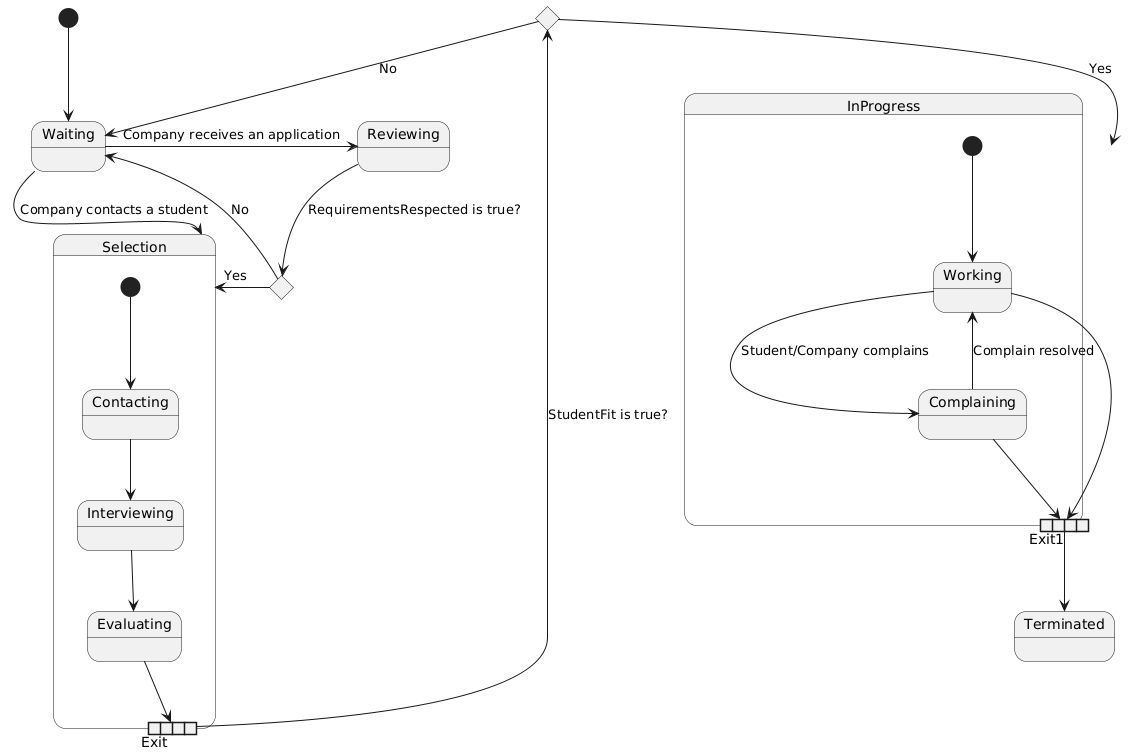
\includegraphics[width=0.8\textwidth]{Assets/Statecharts/Internship_SC.png}
        \caption{Internship state diagram.}
        \label{fig:Internship state diagram.}
    \end{figure}
\textbf{Complaint}\\
There are two ways of complaining, one is by opening the chat section which will permit the student and the company to communicate and resolve minor issues without involving the university. And the other one is by opening the Report Area which is a page where one of the two parties can directly communicate with the university. In this statechart we'll analyze the processes of the second option.
When a user goes to the "Report Area" section it starts the complain process which begins from a Sending state in which the user can write all the reasons of his complain. Once the text is well written and complete the user can send it. Once it is sent, it goes to the Reading state where the complain sent can be read. If it is a termination request, the university, which manages the interruption of the internships, will contact both parties and let them know the collaboration is ended, represented by the Terminated state. Instead if it is a solvable situation, from the Reading state it will arrive in the Resolving state where the parties will start to communicate and try to come up with a solution. If the problem is satisfied, the complain will reach the Solved state and the internship can continue (in the internship statechart it will go back to the Waiting state), instead if a solution isn't found the internship will terminate and the complain will reach the Terminated state.\\
\begin{figure}[H]
        \centering
        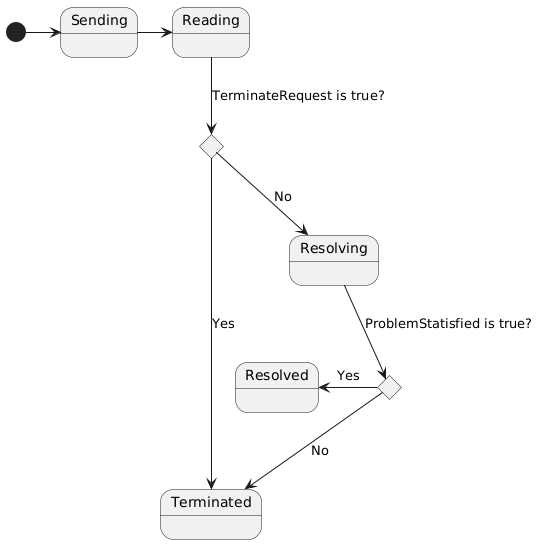
\includegraphics[width=0.8\textwidth]{Assets/Statecharts/Complain_SC.png}
        \caption{Complaint state diagram.}
        \label{fig:Complaint state diagram.}
    \end{figure}
\section{Product Functions}
\subsection{Reccomendation}
The Recommendation Function is a core feature of the S\&C platform that facilitates the matching process between students and companies by suggesting the most suitable opportunities based on the characteristics and preferences of both parties. 
For students the system analyzes their profiles, including their CV, skills, education, work experience, and preferences (e.g., type of internship, location, industry). Based on this data, it creates a personalized homepage where the upper internships showed are the ones that align closely with the student's qualifications and interests.
Instead for companies, the system evaluates the requirements specified in their internship offer, such as required skills, educational background, and job type. It then recommends students whose profiles best meet these criteria, providing companies with a personalized homepage of potential candidates.
The recommendation process uses automated algorithms based on statistical analysis, keyword matching and possibly machine learning to identify relevant matches. Whenever a new student registers to the platform, insert his CV's information and is appetizing for a company, the system will send a notification to the company. The same happens when a company registers and posts an internship offer that might interest a student based on his topic preferences, in this case the system will send a notification to the student and update his homepage. The Recommendation Function ensures that students are connected with internships that suit their career goals while helping companies find candidates who match their needs, creating an efficient and effective matchmaking system.
\subsection{Selection}
The Selection Function is used by companies and manages the steps through which companies evaluate and decide which students are fit to take parts to their internship programs. With this function the platform facilitates the evaluation, interview scheduling, and final selection of candidates in an efficient and organized manner. Is used by companies which firstly review and evaluate students applications. Once they select the student fit for their project they can start by contacting him and through the platform functionalities start to arrange meeting interviews. 
The selection process follows these steps;
1.	Contacting: where companies evaluate and contact the student who sends them an application or directly contact a student that caught their attention in their personalized homepage.
2.	Interviewing: once they select a student they  send him a questionnaire and an interview request to see if he can be fit for their project. 
3. Evaluating: After the interview process if the student is fit, through the contact page offered by the platform they can submit a formal request to start the internship with the selected student.
\section{User charateristics}
\subsection{Student}
The student is a client who is able to access the S\&C platform through the SSO login. They use the platform with the goal of finding an interesting internship project to work on and learn new technologies used in a work environment. Their participation goes through several stages: first they sign into the platform, then they compile a form which asks them various information that will help S\&C to create their CVs. So every time a student wants to contact a company the system will create a personalized CV tailored for the company needs. Each student receives also a notification every time a company posts an announcement on the platform, where the requirements asked fits the ones described by the student in his CV.
\subsection{Company}
The company is a client which represents a business entity that uses the S\&C platform to connect with students that might join their internship project programs. Companies use the platform to contribute to the students growth by offering them a real work experience. Their involvement takes place in several stages: it begins by creating a job opportunity, where they provide the title, a quick description of the internship they are offering, requirements and duration of the internships. They can manage the entire recruitment process through the platform. They can provide feedbacks on the student’s performances during the internship or at the end of it, but more important, they can propose changes to the system to improve the recruitment efficiency. They can also give complaints about the student’s work and ask for the termination of the internship or more likely contact the university to ensure that the issues arising during the internship are addressed effectively. Each company receive a notification every time a student with the correct attributes for their project registers to the platform. The involvement of the companies helps strengthen the connection between schools and the workplace.
\subsection{University}
The university is a client that monitor and support students during their internship. Its role is to ensure that student's learning experiences align with their educational goals and that internships meet the required standards. But also that their students are doing their job in a meticulous way, by being notified from the companies when something doesn’t add up. Their involvement consists in  monitoring student's progress during the internship and ensure that the experience provides meaningful learning opportunities. They are also responsible for handling complaints or issues that may arise during the internship, including resolving cases that require the internship to be interrupted.
\section{Assumptions dependencies and constrains}


\chapter{Specific Requirements}
\section{External Interface Requirements}

\subsection{User Interfaces}
\begin{figure}[H]
      \centering
      
\includegraphics[width=\textwidth]{RASD/Assets/User interfaces/login.png}
      \caption{Login page}
      \label{fig:Login page}
\end{figure}
\begin{figure}[H]
      \centering
      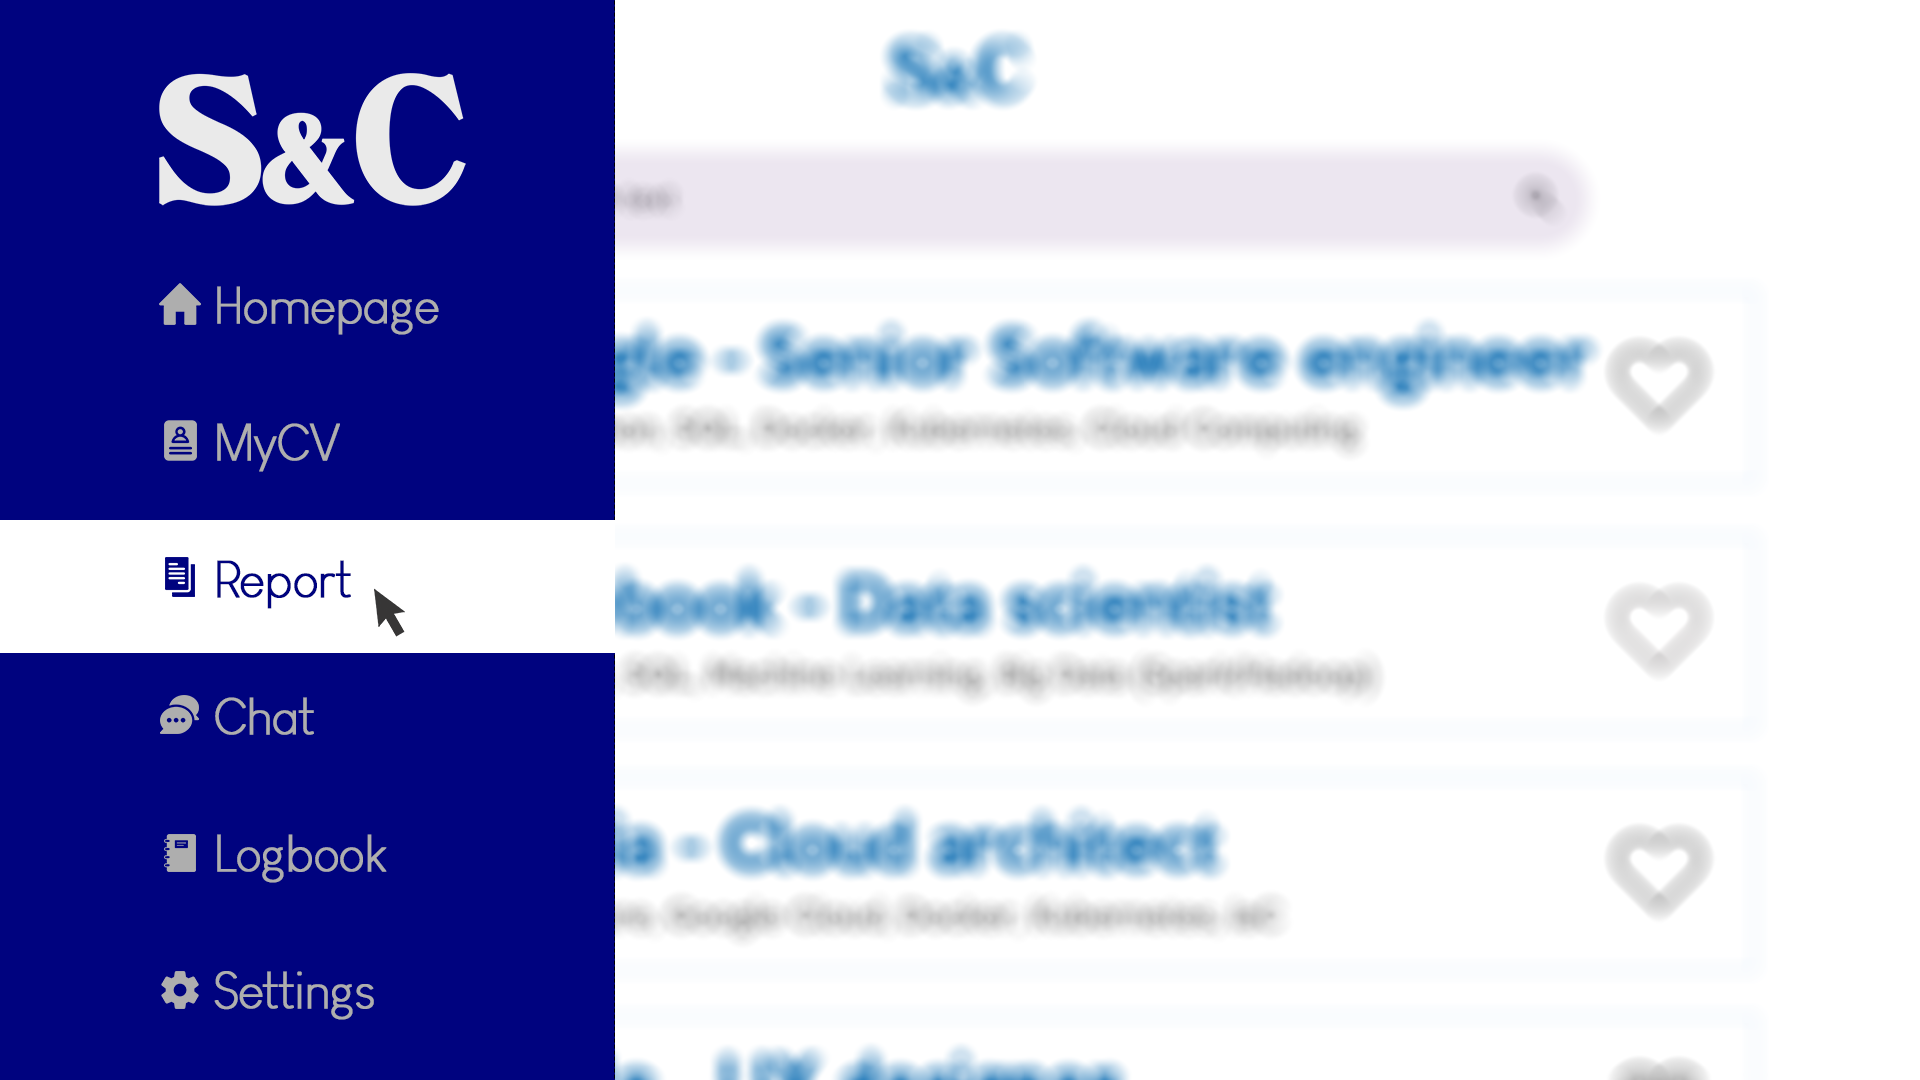
\includegraphics[width=\textwidth]{RASD/Assets/User interfaces/sidebar.png}
      \caption{Student Sidebar}
      \label{fig:Student Sidebar}
\end{figure}
\begin{figure}[H]
      \centering
      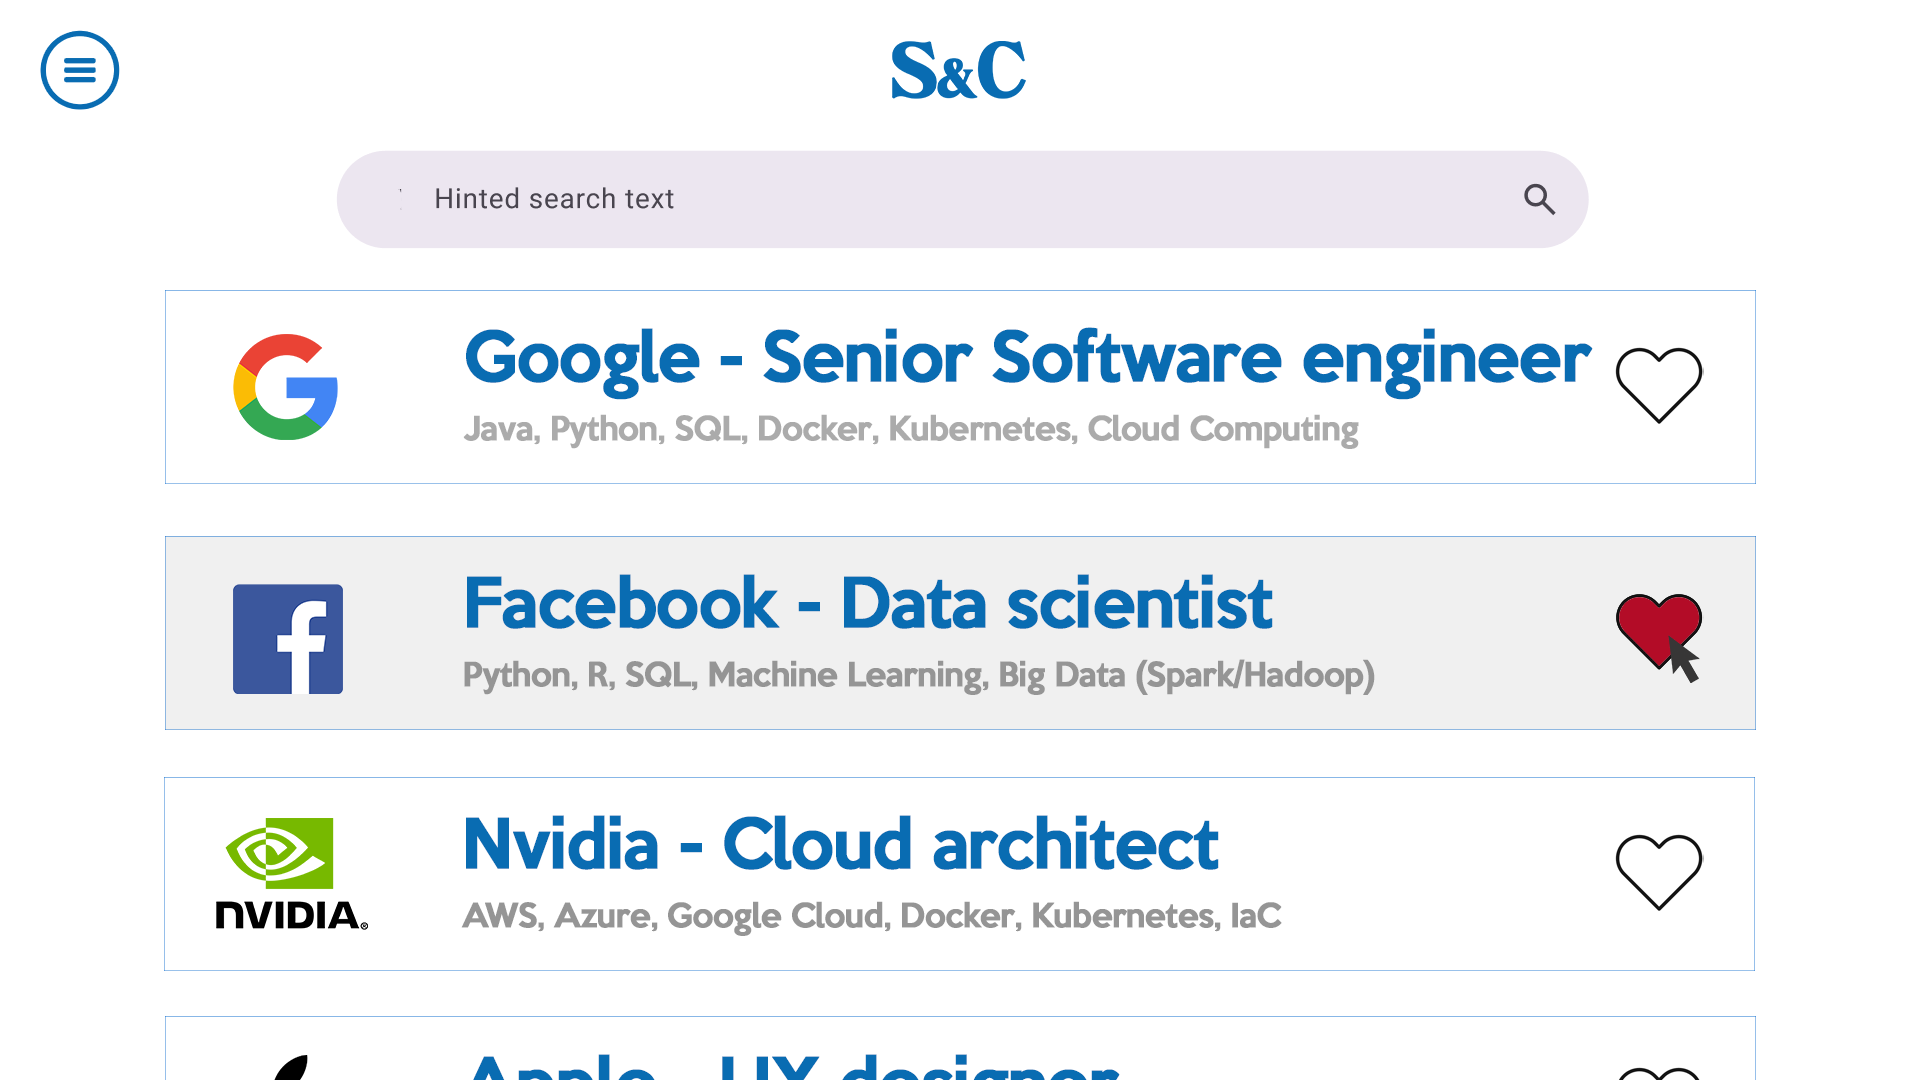
\includegraphics[width=\textwidth]{RASD/Assets/User interfaces/Homepage_student.png}
      \caption{HomePage Student}
      \label{fig:HomePage Student}
\end{figure}
\begin{figure}[H]
      \centering
      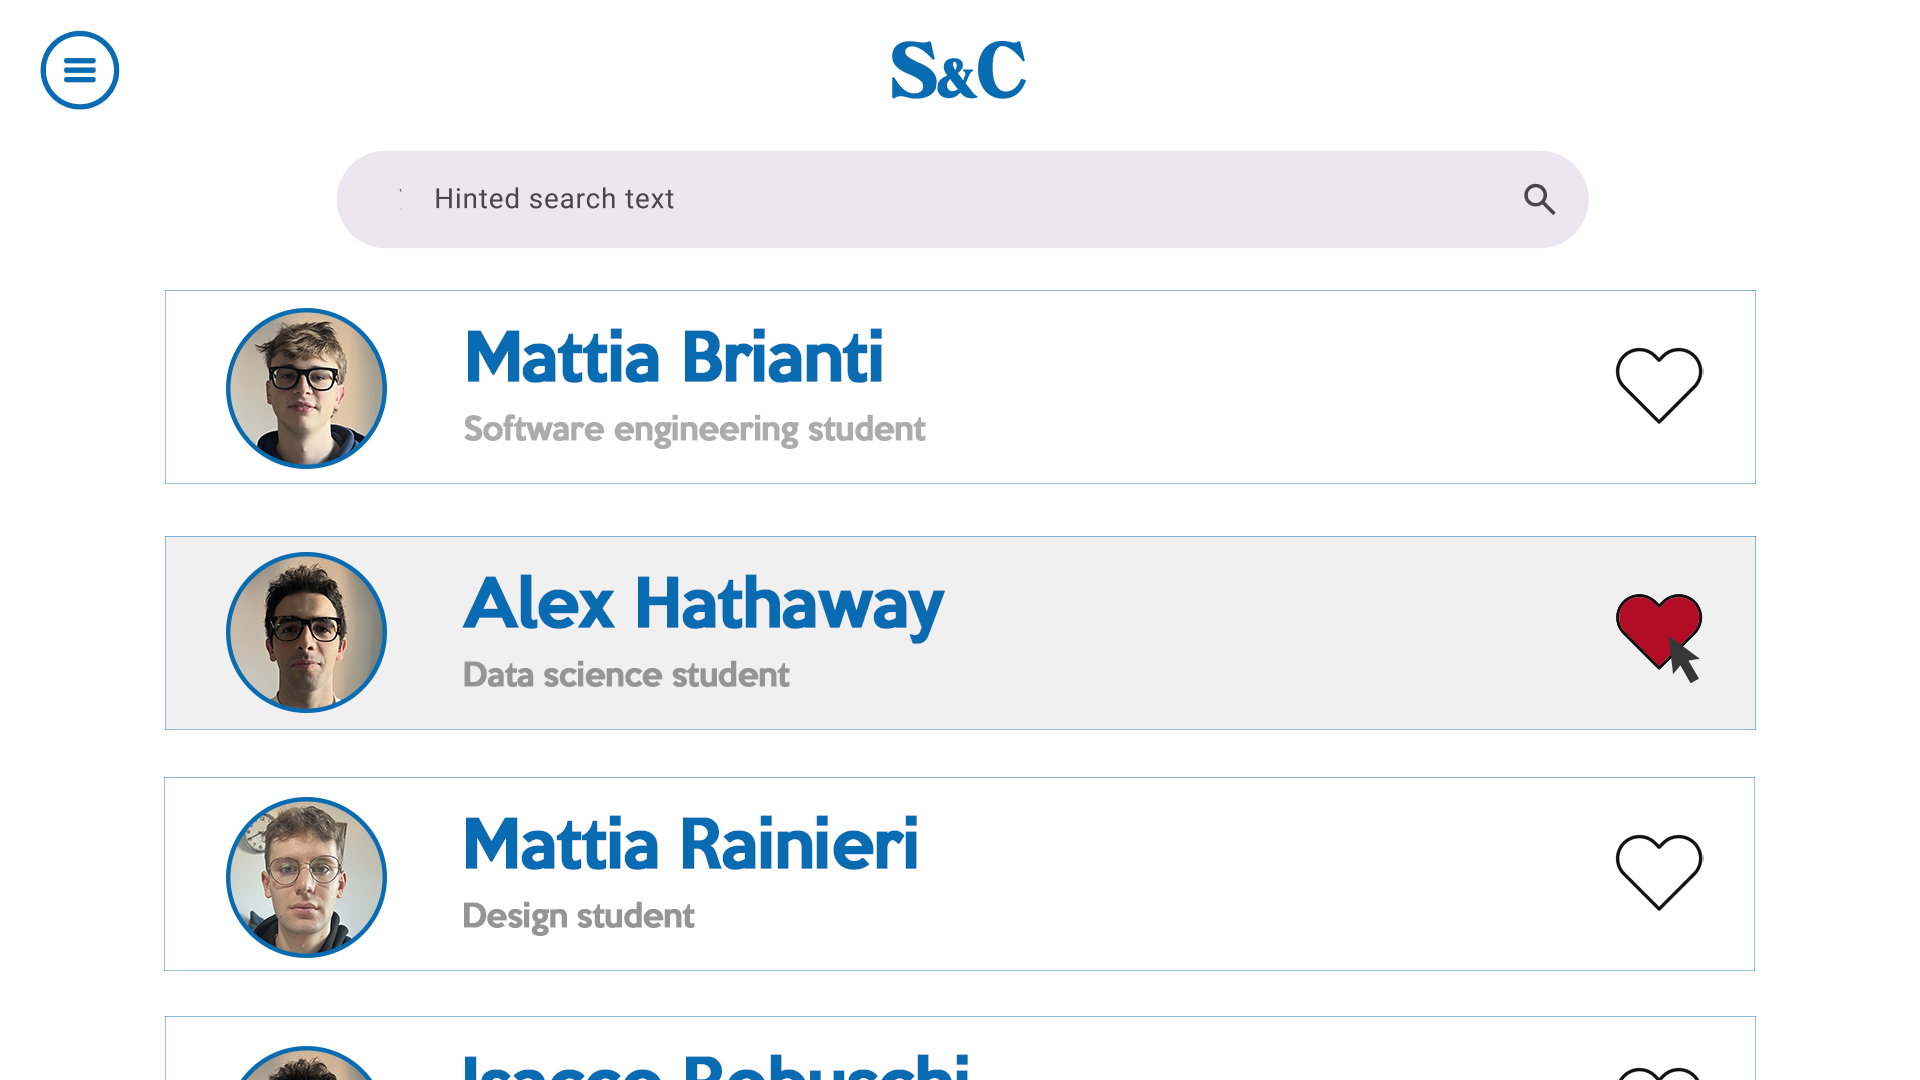
\includegraphics[width=\textwidth]{RASD/Assets/User interfaces/Homepage Company.png}
      \caption{HomePage Company}
      \label{fig:HomePage Company}
\end{figure}


\subsection{Hardware Interfaces}
The system does not need any specific hardware, each user will need a browser with an Internet connection in order to communicate with the servers of the platform.

\subsection{Software Interfaces}
\begin{enumerate}
    \item \textbf{Videocall meeting}
    \item \textbf{AI tool for match making}
    \item \textbf{Databases Interface}
\end{enumerate}

\subsection{Comunication Interfaces}
\begin{enumerate}
    \item \textbf{eduGAIN Radius} - in order to allow a native single sign-on for all European universities.
    \item \textbf{OAuth2} - is a very commonly used standard in the enterprise environment, to consent the adoption of Single Sign On (SSO) with external platform.
    \item \textbf{HyperText Transfer Protocol over Secure Socket Layer (HTTPS)} - used for all communications between client  and server.
    \item \textbf{Simple Mail Transfer Protocol (SMTP)} - , a standard protocol for email transmission, which is used by this platform to send notifications through email.
\end{enumerate}

\section{Functional Requirements}
\begin{enumerate}[label=\textbf{R\arabic*}:,ref=R\arabic*,leftmargin=1.3cm]
    \labelleditem{The system shall allow users to log in with SSO.}
    \labelleditem{The system shall allow the student to provide information for their CVs.}
        \begin{enumerate}[label=\textbf{R\arabic{enumi}.\arabic*}:,ref=R\arabic{enumi}.\arabic*, leftmargin=*]
            \labelledsubitem{The system shall allow the students to specify their personal information, like name, contact and personal ambition.}
            \labelledsubitem{The system shall allow the students to specify their education experience, like the academic background.}
            \labelledsubitem{The system shall allow the students to specify their passed work experience, specifying job title, company name, duration and technologies used.}
            \labelledsubitem{The system shall allow the students to specify their technical and soft skills.}
            \labelledsubitem{The system shall allow the students to specify their project and research, including the title, duration and description}
            \labelledsubitem{The system shall allow the students to specify their extracurricular activities, including the name, organization and achievements.}
            \labelledsubitem{The system shall allow the students to specify their knowledge of languages, including the level and eventual certifications.}
            \labelledsubitem{The system shall allow the students to specify their availability.}
            \labelledsubitem{The system shall allow the students to specify their additional information.}
        \end{enumerate}
    \labelleditem{The system shall allow the students to join an internship.}
        \begin{enumerate}[label=\textbf{R\arabic{enumi}.\arabic*}:,ref=R\arabic{enumi}.\arabic*, leftmargin=*]
            \labelledsubitem{The system shall help the students to create a customized CV for each company.}
        \end{enumerate}
   \labelleditem{The system shall allow the students to be notified when a new interesting internship becomes available.}
    \labelleditem{The system shall allow the company employee to create an internship.}
        \begin{enumerate}[label=\textbf{R\arabic{enumi}.\arabic*}:,ref=R\arabic{enumi}.\arabic*, leftmargin=*]
            \labelledsubitem{The system shall allow the company employee to specify the title of the internship.}
            \labelledsubitem{The system shall allow the company employee to specify the description, helped by an AI, of the internship.}
            \labelledsubitem{The system shall allow the company employee to specify the requirement of the internship.}
            \labelledsubitem{The system shall allow the company employee to specify the duration of the internship.}
            \labelledsubitem{The system shall allow the company employee to specify the availability of the internship.}
            \labelledsubitem{The system shall allow the company employee to specify other information about the internship.}
        \end{enumerate}
    \labelleditem{The system shall allow the company employee to be notified when a new probably interesting student becomes available.}
    \labelleditem{The system shall allow the student to view a personalized homepage after inserting his CV's information.}
    \labelleditem{The system shall allow the company employee to view a personalized homepage after publishing an internship.}
    \labelleditem{The system shall allow the company to write a complaint to the university.}
    \labelleditem{The system shall allow the students to write a complaint to the university.}
    \labelleditem{}{The system shall allow students to chat with his company.}
    \labelleditem{The system shall allow companies employee to chat with his trainee.}
    \labelleditem{The system shall allow universities employee to chat with his students.}
    \labelleditem{The system shall allow the student to insert initial information.}
    \labelleditem{The system shall allow the student and the company to arrange a meeting.}
    \labelleditem{The system shall send a meeting link for the interview to the student and the company.}
    \labelleditem{The system shall allow the student to write on a logbook to inform the university on the status of his internship.}
\end{enumerate}

\subsection{Use case diagrams}
    \subsubsection{Student}

    \begin{figure}[H]
        \centering
        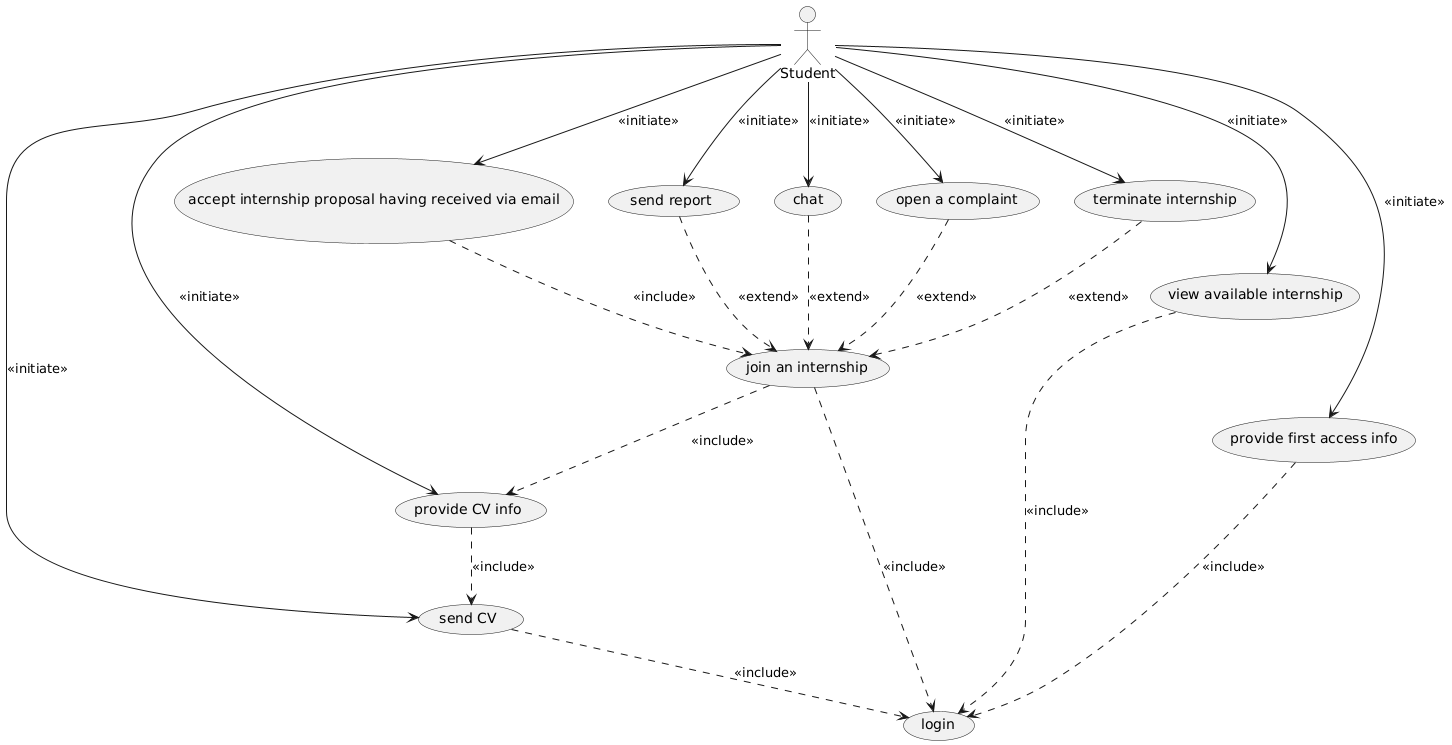
\includegraphics[width=0.8\textwidth]{RASD/Assets/UseCaseDiagram/student.png}
        \caption{Student's use case diagram.}
        \label{fig:Student's use case diagram}
    \end{figure}

\subsubsection{Company employee}

    \begin{figure}[H]
        \centering
        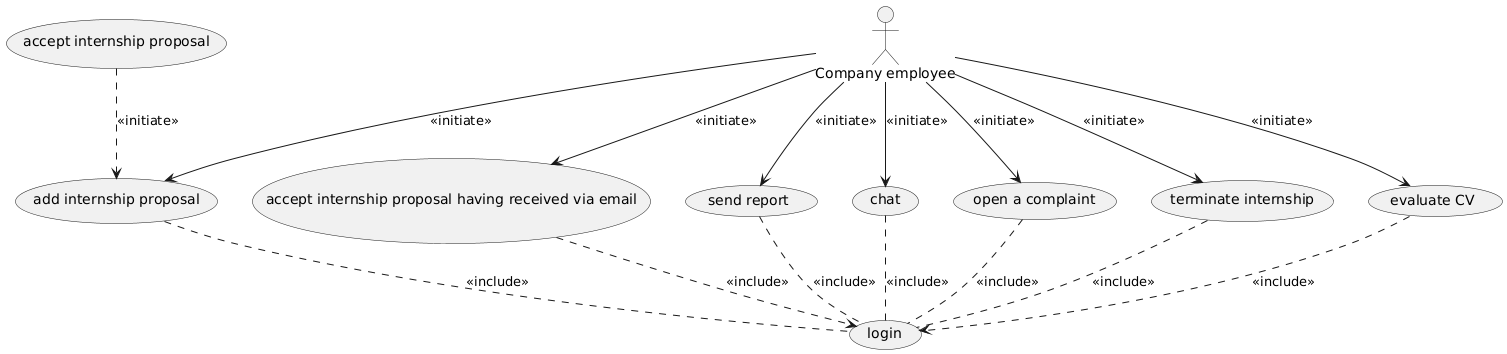
\includegraphics[width=0.8\textwidth]{RASD/Assets/UseCaseDiagram/company.png}
        \caption{Company employee's use case diagram.}
        \label{fig:Company employee's use case diagram}
    \end{figure}

\subsubsection{University employee}

    \begin{figure}[H]
        \centering
        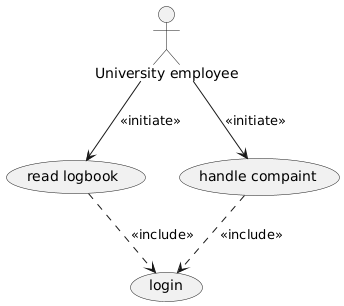
\includegraphics[width=0.8\textwidth]{RASD/Assets/UseCaseDiagram/university.png}
        \caption{University employee's use case diagram.}
        \label{fig:University employee's use case diagram}
    \end{figure}

\pagebreak
\subsection{Use cases}

    \textbf{UC1}
    \begin{table}[H]
    \centering
    \begin{tabular}{|l|p{11.9cm}|}
        \hline
        \textbf{Name}            & Student's first platform access                     \\\hline
        \textbf{Actor}           & Student         \\\hline
        \textbf{Entry condition} &
        \begin{itemize}
              \item Student has never accessed the platform
        \end{itemize}                                        \\\hline
        \textbf{Event flow}      &
        \begin{enumerate}[label=\arabic*.]
              \item The student, who has got an internet connection, insert the URL in the browser.
              \item The student clicks on the login button.
              \item The student inserts his email and will be redirected to the university SSO.
              \item The students selects his favorite academic interests.
        \end{enumerate}            \\\hline
        \textbf{Exit condition}  & The students is redirected to the homepage\\\hline
        \textbf{Exception}       &  Student's credentials are not valid. In this case a pop up will be shown.   \\\hline
    \end{tabular}
    \caption{Student's first platform access}
    \label{table:Student's first platform access}
    \end{table}

    \begin{figure}[H]
        \centering
        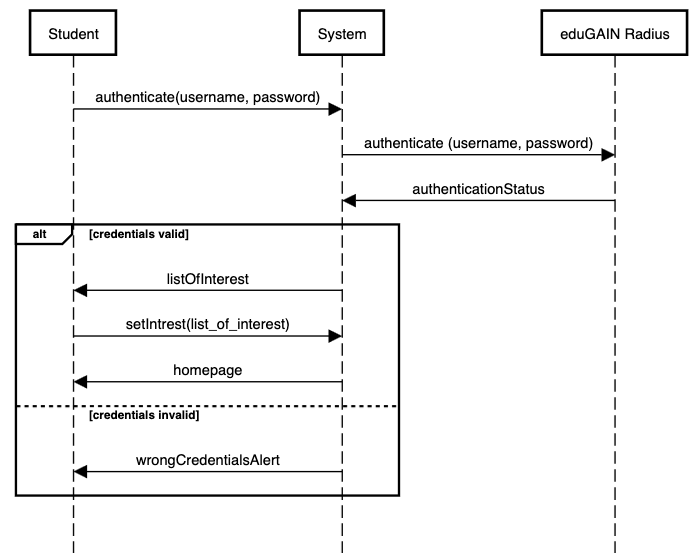
\includegraphics[width=0.8\textwidth]{Assets/SequenceDiagrams/1-login.png}
        \caption{Student's first platform access.}
        \label{fig:Student's first platform access}
    \end{figure}


    \textbf{UC2}
    \begin{table}[H]
    \centering
    \begin{tabular}{|l|p{11.9cm}|}
        \hline
        \textbf{Name}            & Student inserts his CV information in the InitialForm
        \\\hline
        \textbf{Actor}           & Student         \\\hline
        \textbf{Entry condition} &
        \begin{itemize}
              \item Student is already logged in
              \item Student has never provided his information in "My CV" section
        \end{itemize}                                        \\\hline
        \textbf{Event flow}      &
        \begin{enumerate}[label=\arabic*.]
            \item The student press on the contact button.
            \item The student, altered by a pop-up, follows the redirect to the "My CV" page.
            \item The student fills out the form.
            \item The student click on the save button.
        \end{enumerate}            \\\hline
        \textbf{Exit condition}  & The system will show a message confirming the success of the operation.\\\hline
        
        \textbf{Exception}       &  Student misses to compile some fields. In this case, an alert pop-up is shown.  \\\hline
    \end{tabular}
    \caption{Student provides his CV’s information to the platform.}
    \label{table:Student provides his CV’s information to the platform}
    \end{table}

    \begin{figure}[H]
        \centering
        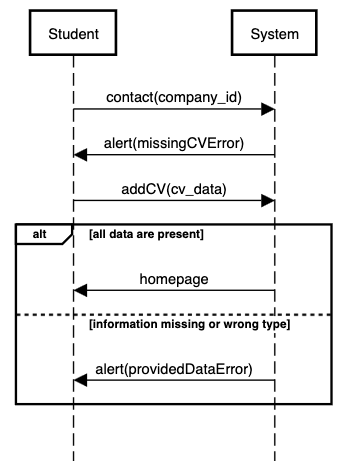
\includegraphics[width=0.8\textwidth]{RASD/Assets/SequenceDiagrams/2-student-provide-his-cv.png}
        \caption{Student provides his CV’s information to the platform.}
        \label{fig:Student provides his CV’s information to the platform}
    \end{figure}


    \textbf{UC3}
    \begin{table}[H]
    \centering
    \begin{tabular}{|l|p{11.9cm}|}
        \hline
        \textbf{Name}            & Student search and contact the company \\\hline
        \textbf{Actor}           & Student, Company Employee         \\\hline
        \textbf{Entry condition} &
        \begin{itemize}
              \item Student is already logged in
              \item Student has already compiled his Curriculum Vitae
        \end{itemize}                                        \\\hline
        \textbf{Event flow}      &
        \begin{enumerate}[label=\arabic*.]
              \item The student opens the homepage.
              \item The student click on contact button next to the interested company.
              \item The platform generate a customized CV.
              \item The student reads the proposal customized and send it.
              \item The company receive the customized CV.
        \end{enumerate}            \\\hline
        \textbf{Exit condition}  & The company employee approve student's CV.\\\hline
        \textbf{Exception}       &  
        \begin{itemize}
              \item The student does not appreciate the customized CV proposed by the platform. In this case, the student manually modify it.
              \item The company employee does not approve the student's CV. In this case, the employee can reject the proposal.  
        \end{itemize} 
        \\\hline
    \end{tabular}
    \caption{Student search and contact the company}
    \label{table:Student search and contact the company}
    \end{table}

    \begin{figure}[H]
        \centering
        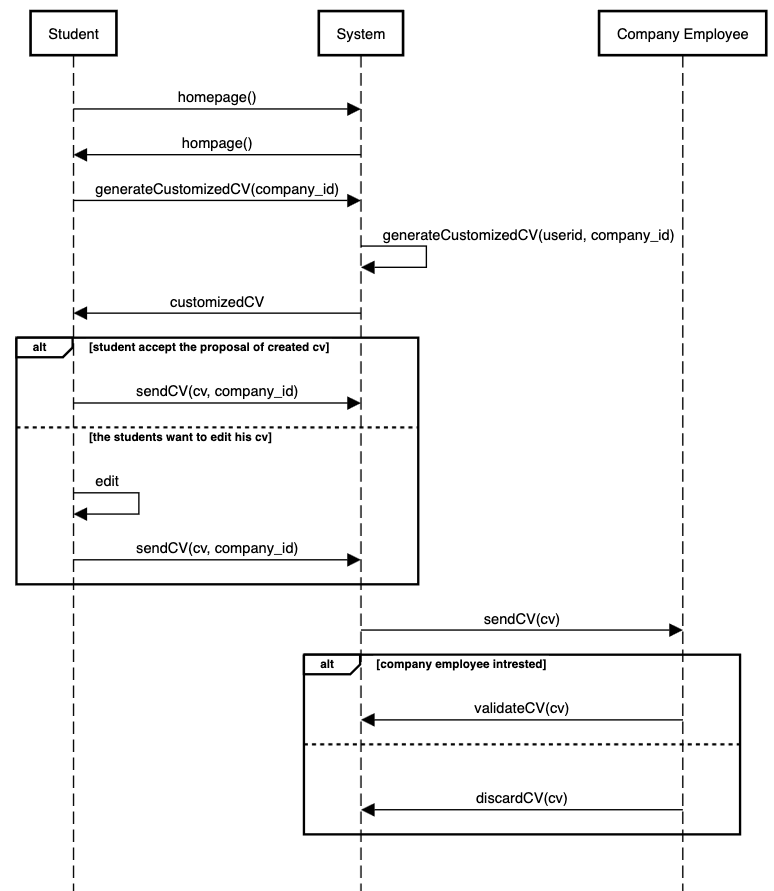
\includegraphics[width=0.8\textwidth]{RASD/Assets/SequenceDiagrams/3-student-contact-company.png}
        \caption{Student search and contact the company.}
        \label{fig:Student search and contact the company}
    \end{figure}
    

    \textbf{UC4}
    \begin{table}[H]
    \centering
    \begin{tabular}{|l|p{11.9cm}|}
        \hline
        \textbf{Name}            & A company publishes an advertisement about the internships they are
offering \\\hline
        \textbf{Actor}           & Company Employee, Student possibly interested on that opportunity.        \\\hline
        \textbf{Entry condition} &
        \begin{itemize}
              \item Company was already approved on the platform
        \end{itemize}                                        \\\hline
        \textbf{Event flow}      &
        \begin{enumerate}[label=\arabic*.]
              \item The company employee logs in using his company's credentials.
              \item The company employee opens the "Create Job Opportunity" page.
              \item The company employee insert into the platform all the information requested.
              \item A successful message is show, and, after a couple of second, the company employee is redirected to the hompage.
        \end{enumerate}            \\\hline
        \textbf{Exit condition}  & Interested students receive a notification \\\hline
        \textbf{Exception}       &  Company employee has not full field the form. In this case, an alert message is shown.   \\\hline
    \end{tabular}
    \caption{Student search and contact the company}
    \label{table:Student search and contact the company}
    \end{table}

    \begin{figure}[H]
        \centering
        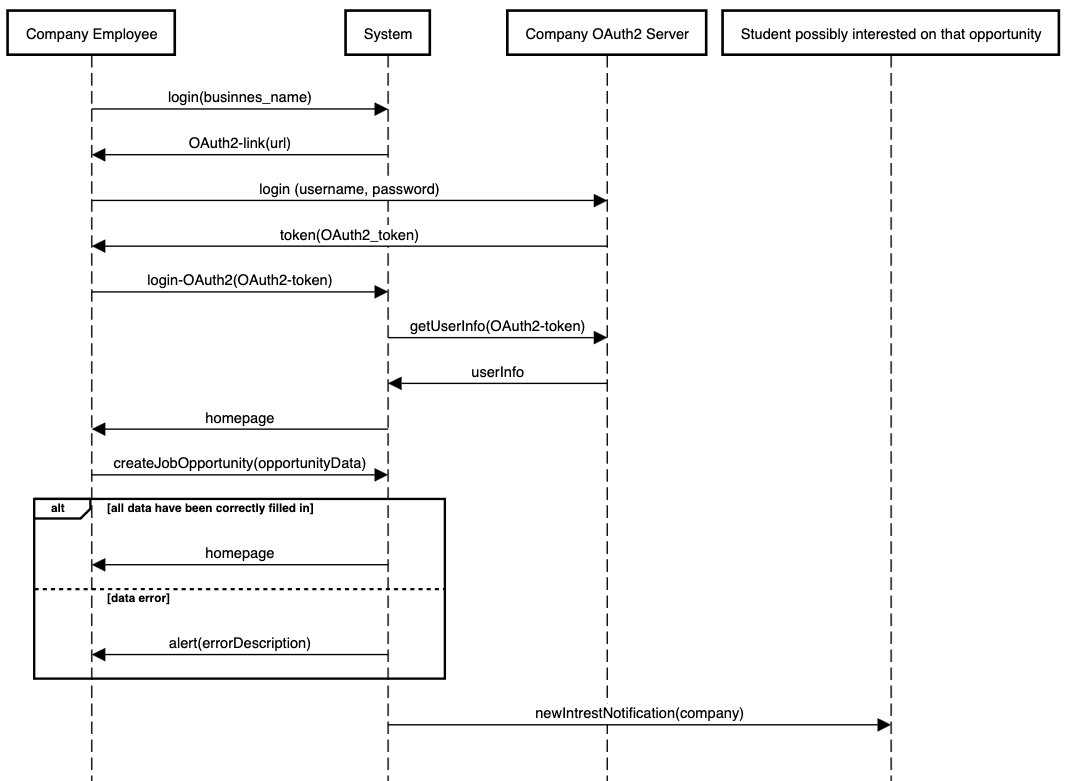
\includegraphics[width=0.8\textwidth]{RASD/Assets/SequenceDiagrams/4-company-publish-and-adv.png}
        \caption{Student search and contact the company.}
        \label{fig:Student search and contact the company}
    \end{figure}


    \textbf{UC5}
    \begin{table}[H]
    \centering
    \begin{tabular}{|l|p{11.9cm}|}
        \hline
        \textbf{Name}            & Student search through the internships and contact the company \\\hline
        \textbf{Actor}           & Student, Company Employee         \\\hline
        \textbf{Entry condition} &
        \begin{itemize}
              \item Student is already logged in
              \item Student has already compiled his Curriculum Vitae
              \item A Company has published an internship that may interest the student.
        \end{itemize}                                        \\\hline
        \textbf{Event flow}      &
        \begin{enumerate}[label=\arabic*.]
              \item The student receive an email.
              \item The student click on the link contained in the email.
              \item The student is interested on that specific internship, so he press on "Contact" button.
              \item The student appreciates the custom generated CV.
        \end{enumerate}            \\\hline
        \textbf{Exit condition}  & Student clicks the "Send" button.\\\hline
        \textbf{Exception}       &  
        \begin{itemize}
            \item The student is not interested on the proposed internship. In this case, the student just ignore the notification.
            \item The student does not appreciate the customized CV proposed by the platform. In this case, the student manually modify it.
        \end{itemize} 
        \\\hline
    \end{tabular}
    \caption{Student search through the internships and contact the company}
    \label{table:Student search through the internhisps and contact the company}
    \end{table}
oi
    \begin{figure}[H]
        \centering
        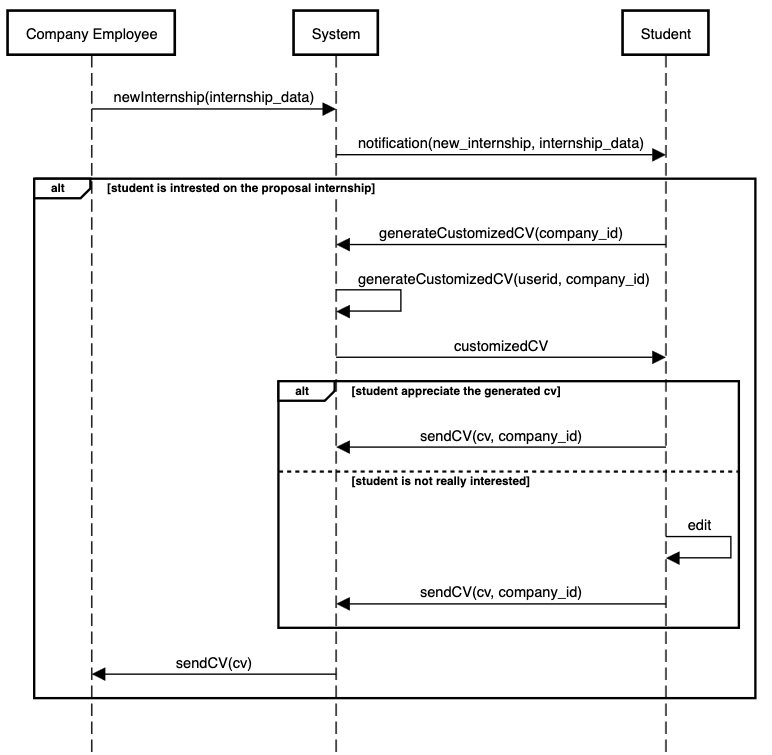
\includegraphics[width=0.8\textwidth]{RASD/Assets/SequenceDiagrams/5-student-receives-a-notification.png}
        \caption{Student receive a notification about the availability of an internship that might interest him.}
        \label{fig:Student receive a notification about the availability of an internship that might interest him}
    \end{figure}

    \textbf{UC6}
    
    \begin{table}[H]
        \centering
        \begin{tabular}{|l|p{11.9cm}|}
        \hline
        \textbf{Name}            & A company receive a notification about the availability of a student CV corresponding to their needs \\\hline
        \textbf{Actor}           & Student, Company Employee       \\\hline
        \textbf{Entry condition} &
        \begin{itemize}
              \item Students has just completed his "My CV" section
        \end{itemize}                                        \\\hline
        \textbf{Event flow}      &
        \begin{enumerate}[label=\arabic*.]
              \item The system will start a matchmaking process between the student and opened internship positions.
              \item The system sends a notification to all of the company employees who may be interested in the new student.
              \item The company employee, who receive the notification, click on the "View Profile" button to obtain more detailed information about his CV.
              \item The company employee click on sends message, near the student name, to contact him.
              
        \end{enumerate}            \\\hline
        \textbf{Exit condition}  & The company employee send a message to the student  \\\hline
        \textbf{Exception}       &  The company employee does not really feel interested in the student's proposal. In this case, he just ignored the mail.   \\\hline
        \end{tabular}
        \caption{A company receive a notification about the availability of a student CV corresponding to their needs.}
        \label{table:A company receive a notification about the availability of a student CV corresponding to their needs}
    \end{table}

    \begin{figure}[H]
        \centering
        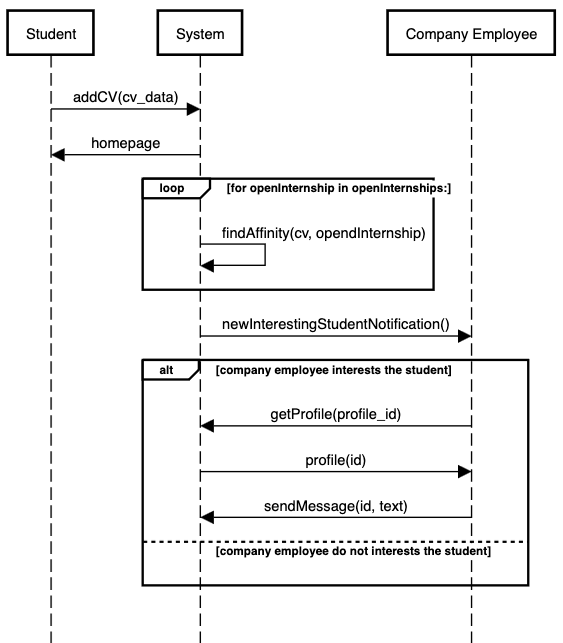
\includegraphics[width=0.8\textwidth]{RASD/Assets/SequenceDiagrams/6-matchmaking-new-student.png}
        \caption{A company receive a notification about the availability of a student CV corresponding to their needs.}
        \label{fig:A company receive a notification about the availability of a student CV corresponding to their needs}
    \end{figure}


    \textbf{UC7}
    
    \begin{table}[H]
        \centering
        \begin{tabular}{|l|p{11.9cm}|}
        \hline
        \textbf{Name}            & Student gives final feedback about the internship \\\hline
        \textbf{Actor}           & Student     \\\hline
        \textbf{Entry condition} &
        \begin{itemize}
              \item Student has just finished his internship
        \end{itemize}                                        \\\hline
        \textbf{Event flow}      &
        \begin{enumerate}[label=\arabic*.]
              \item The student opens the sidebar and click on "Report" button.
              \item The system recognizes that he has just finished an internship, so shows the "Give us your final feedback" form.
              \item The student fills the form.
              
        \end{enumerate}            \\\hline
        \textbf{Exit condition}  & Click on "Submit" button  \\\hline
        \textbf{Exception}       &  The student do not want to provide his feedback. In this case, no action are required.   \\\hline
        \end{tabular}
        \caption{Student gives final feedback about the internship.}
        \label{table:Student gives final feedback about the internship}
    \end{table}

    \begin{figure}[H]
        \centering
        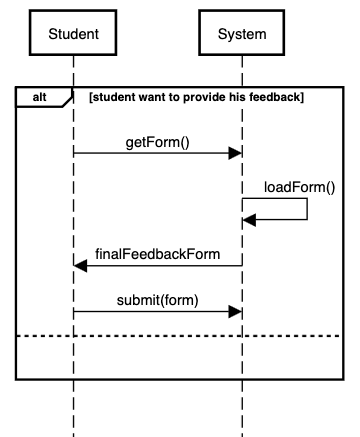
\includegraphics[width=0.8\textwidth]{RASD/Assets/SequenceDiagrams/7-internship-final-form.png}
        \caption{Student gives final feedback about the internship.}
        \label{fig:Student gives final feedback about the internship}
    \end{figure}


    \textbf{UC8}
    
    \begin{table}[H]
        \centering
        \begin{tabular}{|l|p{11.9cm}|}
        \hline
        \textbf{Name}            & University receive the request of ending an internship from a student and contact the company to end it \\\hline
        \textbf{Actor}           & University employee     \\\hline
        \textbf{Entry condition} &
        \begin{itemize}
              \item University employee receives an email 
        \end{itemize}                                        \\\hline
        \textbf{Event flow}      &
        \begin{enumerate}[label=\arabic*.]
              \item The university employee clicks on the "See complain" button in the email, so a new page is opened.
              \item The university employee opens the student's profile by clicking on his name.
              \item The university employee clicks on "Terminate Internship" button.
              
        \end{enumerate}            \\\hline
        \textbf{Exit condition}  & The university employee confirms the pop-up.  \\\hline
        \textbf{Exception}       &    \\\hline
        \end{tabular}
        \caption{University receive the request of ending an internship from a student and contact the company to end it .}
        \label{table:University receive the request of ending an internship from a student and contact the company to end it }
    \end{table}

    \begin{figure}[H]
        \centering
        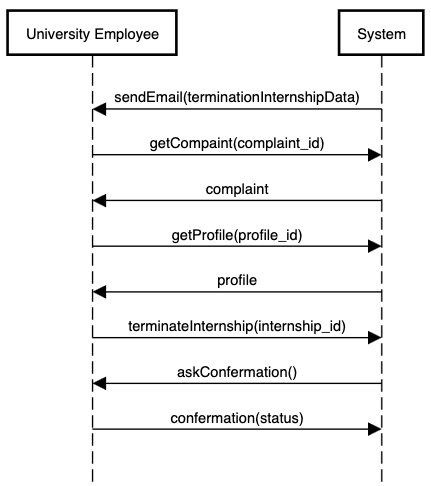
\includegraphics[width=0.8\textwidth]{RASD/Assets/SequenceDiagrams/8-student-end-internship.png}
        \caption{University receive the request of ending an internship from a student and contact the company to end it .}
        \label{fig:University receive the request of ending an internship from a student and contact the company to end it }
    \end{figure}


    \textbf{UC9}
    
    \begin{table}[H]
        \centering
        \begin{tabular}{|l|p{11.9cm}|}
        \hline
        \textbf{Name}            & Student complains with the university on the "Report Area" about his ongoing internship \\\hline
        \textbf{Actor}           & Student    \\\hline
        \textbf{Entry condition} &
        \begin{itemize}
              \item The student is not satisfied with his internship
        \end{itemize}                                        \\\hline
        \textbf{Event flow}      &
        \begin{enumerate}[label=\arabic*.]
              \item The students open the S\&C portal and opens the "Report Area" page.
              \item The student completes the form.
        \end{enumerate}            \\\hline
        \textbf{Exit condition}  & Click on "Submit" button  \\\hline
        \textbf{Exception}       &  The student wants re-try to communicate with his company. In this case, the student will send a message through the chat.   \\\hline
        \end{tabular}
        \caption{Student complains with the university on the "Report Area" about his ongoing internship.}
        \label{table:Student complains with the university on the "Report Area" about his ongoing internship}
    \end{table}

    \begin{figure}[H]
        \centering
        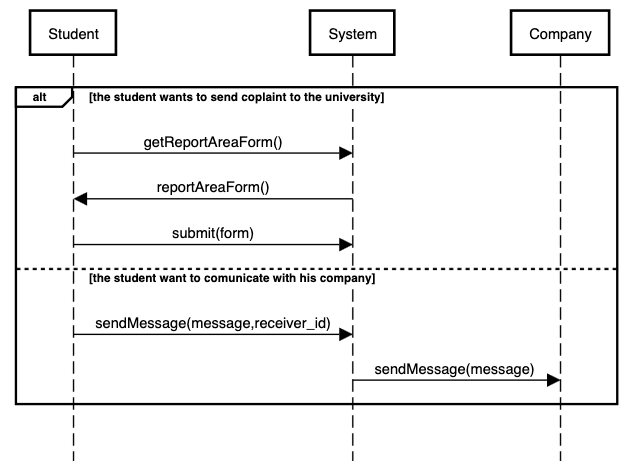
\includegraphics[width=0.8\textwidth]{RASD/Assets/SequenceDiagrams/9-student-sends-a-complaint.png}
        \caption{Student complains with the university on the "Report Area" about his ongoing internship.}
        \label{fig:Student complains with the university on the "Report Area" about his ongoing internship}
    \end{figure}

    \textbf{UC10}
    
    \begin{table}[H]
        \centering
        \begin{tabular}{|l|p{11.9cm}|}
        \hline
        \textbf{Name}            & The company complains about the student taking the internship \\\hline
        \textbf{Actor}           & Company employee, university employee    \\\hline
        \textbf{Entry condition} &
        \begin{itemize}
              \item The company is not satisfied with the student internship
        \end{itemize}                                        \\\hline
        \textbf{Event flow}      &
        \begin{enumerate}[label=\arabic*.]
              \item The company employee open the S\&C portal and opens the "Report Area" page.
              \item The company employee selects the involved student's name.
              \item The company employee clicks on "Report" button in student's page.
              \item The company employee now can fill out the form, describing the problem's detail.
              \item The company employee clicks on "Submit" button
        \end{enumerate}            \\\hline
        \textbf{Exit condition}  & The University receives a notification about the report.\\\hline
        \textbf{Exception}       &  Some form values are missing. In this case, an alert pop-up will be shown.\\\hline
        \end{tabular}
        \caption{The company complains about the student taking the internship.}
        \label{table:The company complains about the student taking the internship}
    \end{table}

    \begin{figure}[H]
        \centering
        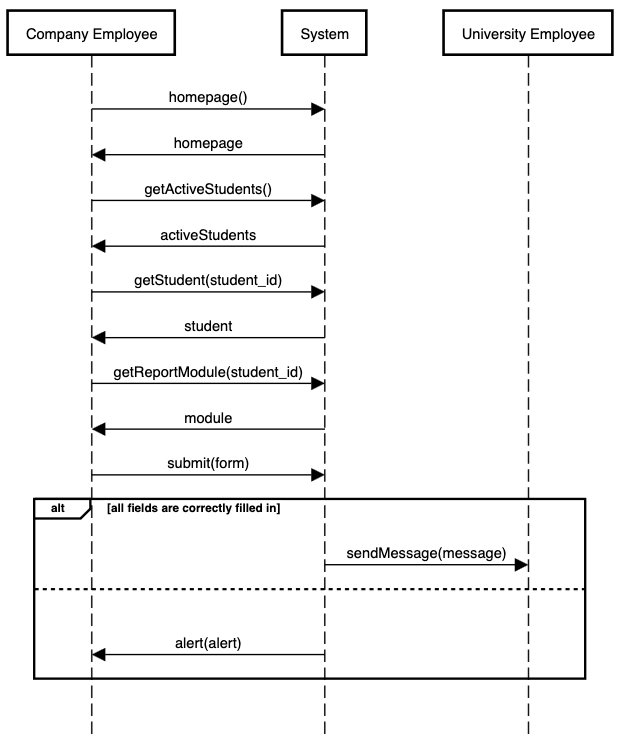
\includegraphics[width=0.8\textwidth]{RASD/Assets/SequenceDiagrams/10-company-sends-a-complaint.png}
        \caption{The company complains about the student taking the internship.}
        \label{fig:The company complains about the student taking the internship}
    \end{figure}

\subsection{Requirements mapping}
In this section it is shown how the $R\land D \models G$ holds.
In particular, the following traceability matrix associates domain assumptions and requirements to goals.
After that, to facilitate reading, the text of all the assumptions and all the requirements related to each goal is reported.
\begin{table}[H]
      %\caption*{\textbf{Title}}
      \centering
      \begin{tabular}{|l|p{8cm}|p{5cm}|}
            \hline
            \textbf{Goal ID} & \textbf{Requirement ID} & \textbf{Domain assumption ID}      \\\hline
            \ref{{G1}}       & \ref{{R1}}, \ref{{R2}}, \ref{{R2.1}}, \ref{{R2.2}}, \ref{{R2.3}}, \ref{{R2.4}}, \ref{{R2.5}}, \ref{{R2.6}}, \ref{{R2.7}}, \ref{{R2.8}}, \ref{{R2.9}}   & \ref{{D1}}, \ref{{D2}}, \ref{{D3}}                
             \\\hline
             
            \ref{{G2}}       & \ref{{R1}}, \ref{{R5}}, \ref{{R5.1}}, \ref{{R5.2}}, \ref{{R5.3}}, \ref{{R5.4}}, \ref{{R5.5}}, \ref{{R5.6}}
            & \ref{{D1}}, \ref{{D2}}, \ref{{D3}}     \\\hline
            
            \ref{{G3}}
            &
            \ref{{R1}}, \ref{{R5}},\ref{{R5.2}}, \ref{{R5.3}}, \ref{{R5.4}}, \ref{{R5.5}}, \ref{{R5.6}} \ref{{R13}}  
            & 
            \ref{{D1}}, \ref{{D2}}, \ref{{D3}}, \ref{{D6}}, \ref{{D8}}  \\\hline
            
            \ref{{G4}}
            & 
            \ref{{R1}}, \ref{{R4}}, \ref{{R5}}, \ref{{R5.1}}, \ref{{R5.2}}, \ref{{R5.3}}, \ref{{R5.4}}, \ref{{R5.5}}, \ref{{R5.6}}
            & 
            \ref{{D1}}, \ref{{D2}}, \ref{{D3}}, \ref{{D6}}                                \\\hline

            
            \ref{{G5}}       
            &
            \ref{{R1}}, \ref{{R2}}, \ref{{R2.1}}, \ref{{R2.2}}, \ref{{R2.3}}, \ref{{R2.4}}, \ref{{R2.5}}, \ref{{R2.6}}, \ref{{R2.7}}, \ref{{R2.8}}, \ref{{R2.9}}, \ref{{R5}}, \ref{{R5.1}}, \ref{{R5.2}}, \ref{{R5.3}}, \ref{{R5.4}}, \ref{{R5.5}}, \ref{{R5.6}}, \ref{{R6}}
            & 
            \ref{{D1}}, \ref{{D2}}, \ref{{D3}}, \ref{{D6}}                     
            \\\hline
            
            
            \ref{{G6}}
            &
            \ref{{R1}}, \ref{{R2}}, \ref{{R2.1}}, \ref{{R2.2}}, \ref{{R2.3}}, \ref{{R2.4}}, \ref{{R2.5}}, \ref{{R2.6}}, \ref{{R2.7}}, \ref{{R2.8}}, \ref{{R2.9}}, \ref{{R4}}, \ref{{R5}}, \ref{{R5.1}}, \ref{{R5.2}}, \ref{{R5.3}}, \ref{{R5.4}}, \ref{{R5.5}}, \ref{{R5.6}}, \ref{{R6}}, \ref{{R7}}, \ref{{R8}}
            &
            \ref{{D1}}, \ref{{D2}}, \ref{{D3}}, \ref{{D6}}                                \\\hline

            
            \ref{{G7}}
            & 
            \ref{{R1}}, \ref{{R2}}, \ref{{R2.1}}, \ref{{R2.2}}, \ref{{R2.3}}, \ref{{R2.4}}, \ref{{R2.5}}, \ref{{R2.6}}, \ref{{R2.7}}, \ref{{R2.8}}, \ref{{R2.9}}, \ref{{R5}},\ref{{R5.1}}, \ref{{R5.2}}, \ref{{R5.3}}, \ref{{R5.4}}, \ref{{R5.5}}, \ref{{R5.6}}, \ref{{R11}}, \ref{{R12}}
            & 
            \ref{{D1}}, \ref{{D2}}, \ref{{D3}}
            \\\hline

            
            \ref{{G8}}
            &
            \ref{{R1}}, \ref{{R2}}, \ref{{R2.1}}, \ref{{R2.2}}, \ref{{R2.3}}, \ref{{R2.4}}, \ref{{R2.5}}, \ref{{R2.6}}, \ref{{R2.7}}, \ref{{R2.8}}, \ref{{R2.9}}, \ref{{R3}}, \ref{{R5}}, \ref{{R5.1}}, \ref{{R5.2}}, \ref{{R5.3}}, \ref{{R5.4}}, \ref{{R5.5}}, \ref{{R5.6}}, \ref{{R12}}, \ref{{R13}}, \ref{{R15}}, \ref{{R16}}
            &
            \ref{{D1}}, \ref{{D3}}, \ref{{D3}}, 
            \\\hline

            
            \ref{{G9}}
            &
            \ref{{R1}}, \ref{{R2}}, \ref{{R2.1}}, \ref{{R2.2}}, \ref{{R2.3}}, \ref{{R2.4}}, \ref{{R2.5}}, \ref{{R2.6}}, \ref{{R2.7}}, \ref{{R2.8}}, \ref{{R2.9}}, \ref{{R3}}, \ref{{R5}}, \ref{{R5.1}}, \ref{{R5.2}}, \ref{{R5.3}}, \ref{{R5.4}}, \ref{{R5.5}}, \ref{{R5.6}},\ref{{R7}}, \ref{{R17}}
            &
            \ref{{D1}}, \ref{{D2}}, \ref{{D3}}, \ref{{D9}}                                \\\hline

            
            \ref{{G10}}
            &
            \ref{{R1}}, \ref{{R3}}, \ref{{R5}}, \ref{{R5.1}}, \ref{{R5.2}}, \ref{{R5.3}}, \ref{{R5.4}}, \ref{{R5.5}}, \ref{{R5.6}} \ref{{R9}}, \ref{{R10}}, \ref{{R13}}, \ref{{R17}}
            &
            \ref{{D1}}, \ref{{D2}}, \ref{{D3}}, \ref{{D9}}
            \\\hline

            
            \ref{{G11}}
            &
            \ref{{R1}}, \ref{{R3}}, \ref{{R5}}, \ref{{R5.1}}, \ref{{R5.2}}, \ref{{R5.3}}, \ref{{R5.4}}, \ref{{R5.5}}, \ref{{R5.6}},  \ref{{R9}}, \ref{{R12}}
            &
            \ref{{D1}}, \ref{{D2}}, \ref{{D3}}, \ref{{D5}}
            \\\hline
            
            
            \ref{{G12}}
            &
            \ref{{R1}}, \ref{{R2}}, \ref{{R2.1}}, \ref{{R2.2}}, \ref{{R2.3}}, \ref{{R2.4}}, \ref{{R2.5}}, \ref{{R2.6}}, \ref{{R2.7}}, \ref{{R2.8}}, \ref{{R2.9}}, \ref{{R3}}, \ref{{R5}}, \ref{{R5.1}}, \ref{{R5.2}}, \ref{{R5.3}}, \ref{{R5.4}}, \ref{{R5.5}}, \ref{{R5.6}}, \ref{{R10}}, \ref{{R11}}, \ref{{R12}}, \ref{{R13}}
            &
            \ref{{D1}}, \ref{{D2}}, \ref{{D3}}, \ref{{D5}}        \\\hline
            
      \end{tabular}
      \caption{Traceability matrix}
      \label{table:Traceability matrix}
\end{table}

\begin{enumerate}[leftmargin=1.3cm]
    \printitem{G1}
    \begin{enumerate}[leftmargin=1.3cm]
        \printitem{R1}
        \printitem{R2}
        \printitem{R2.1}
        \printitem{R2.2}
        \printitem{R2.3}
        \printitem{R2.4}
        \printitem{R2.5}
        \printitem{R2.6}
        \printitem{R2.7}
        \printitem{R2.8}
        \printitem{R2.9}
        \printitem{D1}
        \printitem{D2}
        \printitem{D3}
    \end{enumerate}
     \printitem{G2}
    \begin{enumerate}[leftmargin=1.3cm]
        \printitem{R1}
        \printitem{R5}
        \printitem{R5.1}
        \printitem{R5.2}
        \printitem{R5.3}
        \printitem{R5.4}
        \printitem{R5.5}
        \printitem{R5.6}
        \printitem{D1}
        \printitem{D2}
        \printitem{D3}
    \end{enumerate}
     \printitem{G3}
    \begin{enumerate}[leftmargin=1.3cm]
        \printitem{R1}
        \printitem{R5}
        \printitem{R5.1}
        \printitem{R5.2}
        \printitem{R5.3}
        \printitem{R5.4}
        \printitem{R5.5}
        \printitem{R5.6}
        \printitem{R13}
        \printitem{D1}
        \printitem{D2}
        \printitem{D3}
        \printitem{D6}
        \printitem{D8}
    \end{enumerate}
    \printitem{G4}
    \begin{enumerate}[leftmargin=1.3cm]
        \printitem{R1}
        \printitem{R4}
        \printitem{R5}
        \printitem{R5.1}
        \printitem{R5.2}
        \printitem{R5.3}
        \printitem{R5.4}
        \printitem{R5.5}
        \printitem{R5.6}
        \printitem{D1}
        \printitem{D2}
        \printitem{D3}
    \end{enumerate}
    \printitem{G5}
    \begin{enumerate}[leftmargin=1.3cm]
        \printitem{R1}
        \printitem{R2}
        \printitem{R2.1}
        \printitem{R2.2}
        \printitem{R2.3}
        \printitem{R2.4}
        \printitem{R2.5}
        \printitem{R2.6}
        \printitem{R2.7}
        \printitem{R2.8}
        \printitem{R2.9}
        \printitem{R5}
        \printitem{R5.1}
        \printitem{R5.2}
        \printitem{R5.3}
        \printitem{R5.4}
        \printitem{R5.5}
        \printitem{R5.6}
        \printitem{D1}
        \printitem{D2}
        \printitem{D3}
        \printitem{D6}
    \end{enumerate}
    \printitem{G6}
    \begin{enumerate}[leftmargin=1.3cm]
        \printitem{R1}
        \printitem{R2}
        \printitem{R2.1}
        \printitem{R2.2}
        \printitem{R2.3}
        \printitem{R2.4}
        \printitem{R2.5}
        \printitem{R2.6}
        \printitem{R2.7}
        \printitem{R2.8}
        \printitem{R2.9}
        \printitem{R5}
        \printitem{R5.1}
        \printitem{R5.2}
        \printitem{R5.3}
        \printitem{R5.4}
        \printitem{R5.5}
        \printitem{R5.6}
        \printitem{R6}
        \printitem{R7}
        \printitem{R8}
        \printitem{D1}
        \printitem{D2}
        \printitem{D3}
        \printitem{D6}
    \end{enumerate}
    \printitem{G7}
    \begin{enumerate}[leftmargin=1.3cm]
        \printitem{R1}
        \printitem{R2}
        \printitem{R2.1}
        \printitem{R2.2}
        \printitem{R2.3}
        \printitem{R2.4}
        \printitem{R2.5}
        \printitem{R2.6}
        \printitem{R2.7}
        \printitem{R2.8}
        \printitem{R2.9}
        \printitem{R5}
        \printitem{R5.1}
        \printitem{R5.2}
        \printitem{R5.3}
        \printitem{R5.4}
        \printitem{R5.5}
        \printitem{R5.6}
        \printitem{R11}
        \printitem{R12}
        \printitem{D1}
        \printitem{D2}
        \printitem{D3}
    \end{enumerate}
\end{enumerate}

\section{Performance Requirements}
The system must be sized according to the number of users who will use it. Since the system operations are pretty lightfull.

\section{Design Constraints}
\subsection{Standards Compliance}
In order to make the software as compatible and secure as possible, the following standards has been chosen: 
\begin{enumerate}
    \item Accessibility Standard
    \item REST Standard
    \item Security Algorithm 
    \item OpenAPI (Swagger).
    \item Privacy
\end{enumerate}


\subsection{Hardware limitations}
Each user must have an electronic device with an Internet connection that allows him/her to access the S\&C website. No particular hardware characteristics are required, but a stable Internet connection and a screen capable of displaying web pages. The device used by the user will allow him/her to view, access and modify the various sections of the platform. It will also be possible to receive notifications directly.
\section{Software System Attributes}
\subsection{Reliability}
The S\&C platform does not manage critical operations. If any operations fail it can be re-executed without any particular consequences. For example, if the submit of an internship request fails, the company can resubmit the request.
\subsection{Availability}
The system should always be available. The only downtime allowed is between 1 am and 5 am when students and employee are usually not studying nor working. The platform shall therefore guarantee 99\% (two-nines) of availability.
\subsection{Security}
Communication between the user and the S\&C platform is encrypted and data are protected by all possible security means to prevent cyber attacks. Furthermore, students cannot access data to which they are not authorised. For instance, they cannot access other students' data or see the logbooks of other internships. Companies are also not allowed to view the data of other companies or their interns.
\subsection{Maintainability}
The system must be divided into modules, which makes it scalable and reusable and therefore easier to maintain and replace in the case of failures. Ordinary maintenance is performed during night hours, when students and workers do not usually access the platform
\subsection{Portability}
The S\&C platform does not need any special hardware or software, as it is easily accessible from any operating system with a web browser. A mobile application could also be developed to make access more immediate

\chapter{Formal analysis using alloy}
This section describes the entire model formally using the alloy language.
In particular, we aim to model the relationships between entities that are used in the management of internships, such as students, companies and universities. Furthermore, we aim to ensure consistency by introducing the constraints that enable the creation and management of all processes in the system


\section{Alloy Code}
\lstinputlisting[language=alloy]{alloy/model.als}
\pagebreak

\section{Models}
\begin{enumerate}[label=,leftmargin=0cm]
      \item \textbf{Student participates in an internship}

            This model was generated using:
            \begin{lstlisting}[language=alloy]
            run {
                #Student = 2
	        #Company = 1
	        #Internship = 1
	        some i: Internship | i.state = InProgress
	        #Preferences >= 4
            } for 10
	
          \end{lstlisting}

            \begin{adjustbox}{max size={\textwidth}{\textheight}}
                  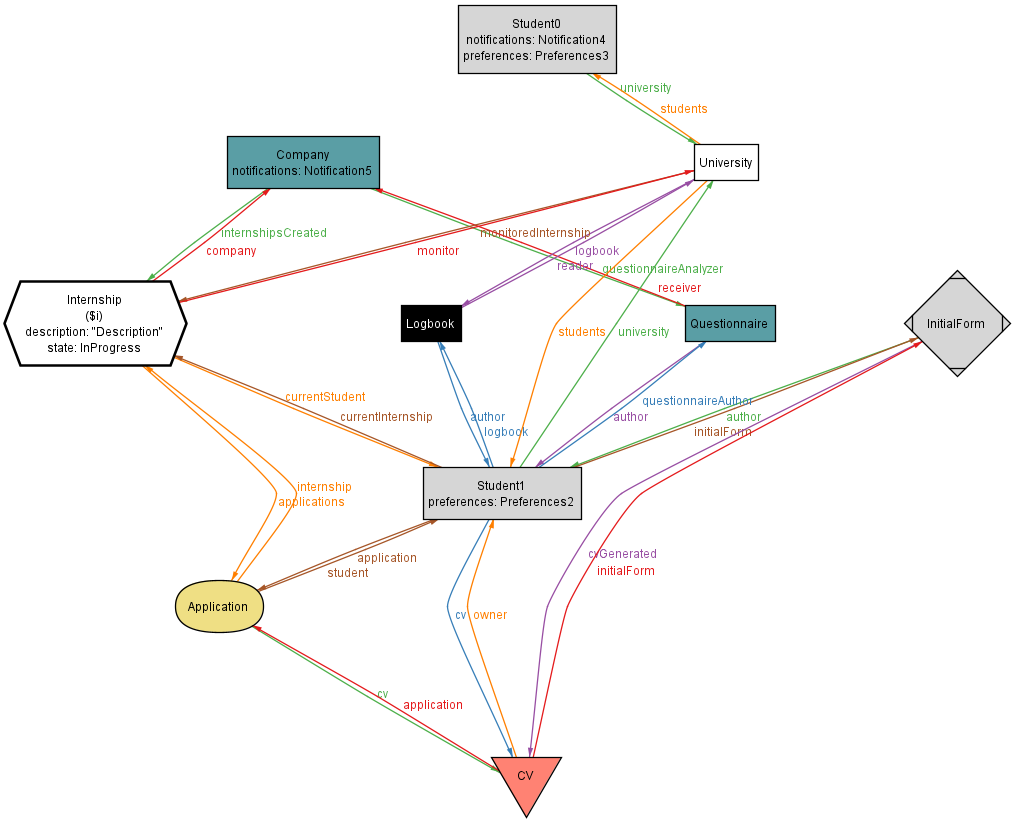
\includegraphics{alloy/alloy1.png}
            \end{adjustbox}

            This diagram shows us 2 students belonging to the same university. One of the two students is doing an internship at a company, and it shows us that this student had to fill out an ‘Initial Form’ in order to produce the CV that was used to make the application. The student also had to fill in a questionnaire at the selection stage and now has a logbook where he notes what he does in the company.

        \pagebreak
        \item \textbf{Company makes a report}

            This model was generated using:
            \begin{lstlisting}[language=alloy]
            run {
	        #Student = 3
	        #Company = 3
                #Internship = 3
                some i: Internship | i.state = InProgress
                #Preferences >= 4
                #ChatMessage >= 1
                #Report = 1
            } for 10
	
          \end{lstlisting}

            \begin{adjustbox}{max size={\textwidth}{\textheight}}
                  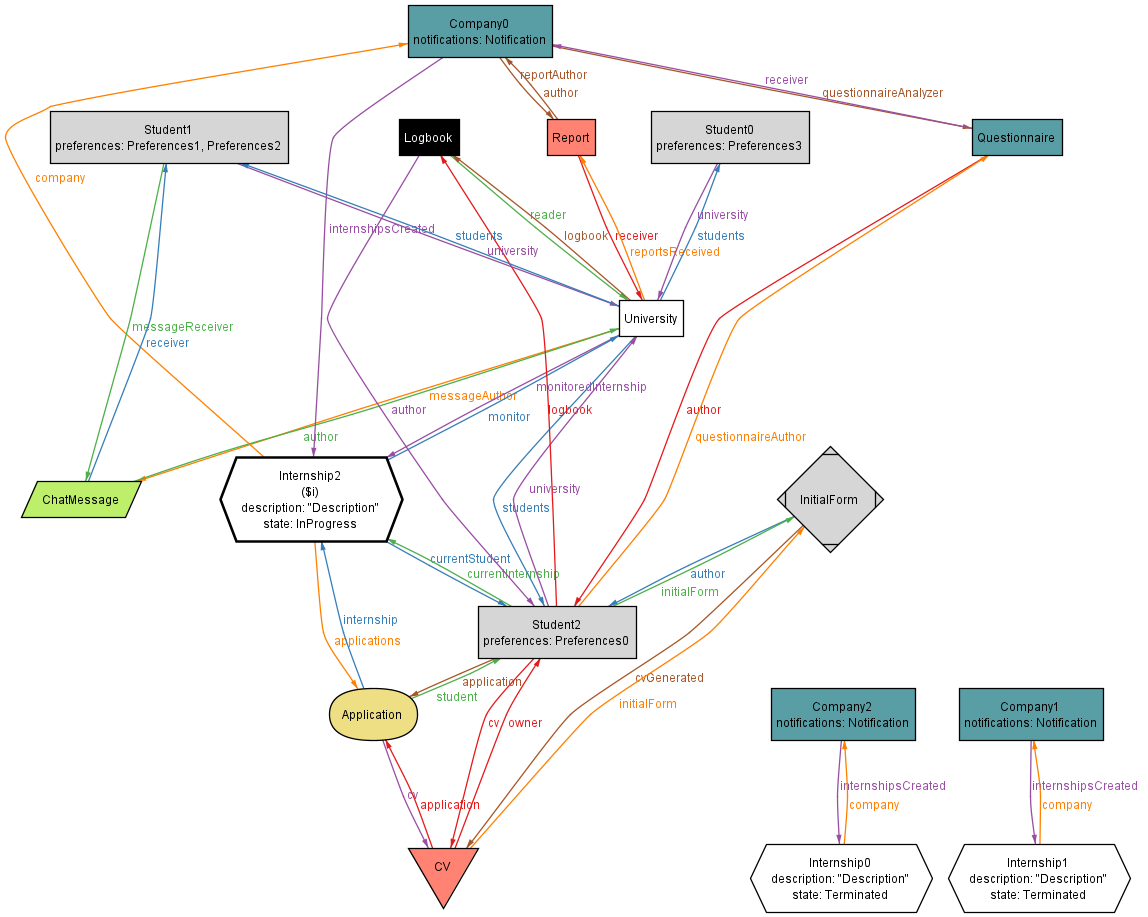
\includegraphics{RASD/alloy/alloy2.png}
            \end{adjustbox}

            This diagram shows us Student2 doing the Internship2, and he has in fact filled in an InitialForm and made the application (thus generating a CV). We also see that Company0, responsible for Internship2 has made a report to the university, probably reporting insufficient work by the student. We also see that Student1 has communicated with his university via chat. Finally, we can see that 2 other companies have created 2 internships which are now both terminated and therefore no longer have students
\end{enumerate}

\chapter{Effort spent}
% !TeX root = ../rasd.tex
\begin{table}[H]
      %\caption*{\textbf{Title}}
      \centering
      \begin{tabular}{|l|l|l|}
            \hline
            \textbf{Member of group }                  & \textbf{Chapter}            & \textbf{Time spent} \\\hline
            \multirow{4}{*}{\textbf{Mattia Brianti}} & Introduction                & 8h                  \\
                                                       & Overall Description         & 0h                \\
                                                       & Specific Requirements       & 0h                 \\
                                                       & Formal analysis using alloy & 5h                 \\\hline
            \multirow{4}{*}{\textbf{Alex Hathaway}} & Introduction                & 0h                  \\
                                                       & Overall Description         & 0h                  \\
                                                       & Specific Requirements       & 0h                  \\
                                                       & Formal analysis using alloy & 0h                  \\\hline
            \multirow{4}{*}{\textbf{Mattia Rainieri}} & Introduction                & 0h                  \\
                                                       & Overall Description         & 0h                 \\
                                                       & Specific Requirements       & 0h                  \\
                                                       & Formal analysis using alloy & 0h                \\\hline
      \end{tabular}
      \caption{Time spent by each member of group.}
      \label{table:Time spent}
\end{table}


%-------------------------------------------------------------------------
%	BIBLIOGRAPHY
%-------------------------------------------------------------------------

\addtocontents{toc}{\vspace{2em}} % Add a gap in the Contents, for aesthetics
\nocite{*}
\bibliography{bibliography}


% LIST OF FIGURES
\listoffigures
% LIST OF TABLES
\listoftables

\cleardoublepage

\end{document}
    